\documentclass[unnumsec,webpdf,contemporary,large]{oup-authoring-template}
%% ---------------------------------------------------------------------------
%% Glaukopis: Cyber Threat Intelligence Language Model Training:
%% Optimizing Domain Specific LLM Performance
%%
%% Worth, Cardei, Alam. Formatted for the OUP contemporary
%% author-year template. Compile with pdfLaTeX.
%%
%% NOTE: This template already loads amsmath, amssymb, hyperref, graphicx,
%% url, natbib, etc. Do NOT re-load them.
%% ---------------------------------------------------------------------------

\graphicspath{{img/}{Fig/}}

%% Theorem-style declarations (OUP-standard; kept for completeness even if unused)
\theoremstyle{thmstyleone}
\newtheorem{theorem}{Theorem}
\newtheorem{proposition}[theorem]{Proposition}
\theoremstyle{thmstyletwo}
\newtheorem{example}{Example}
\newtheorem{remark}{Remark}
\theoremstyle{thmstylethree}
\newtheorem{definition}{Definition}

\begin{document}

\journaltitle{Journal of Cybersecurity}
\DOI{DOI added during production}
\copyrightyear{2026}
\pubyear{2026}
\vol{XX}
\issue{x}
\access{Published: Date added during production}
\appnotes{Paper}

\firstpage{1}

\title[Glaukopis: A Small (32B) CTI LLM via Instruction Finetuning]{Glaukopis: Using Instruction Finetuning to Create a Small (32B) CTI LLM}

\author[1,$\ast$]{Peter J. Worth Jr.}
\author[1]{Ionut Cardei}
\author[1]{Md Tanvirul Alam}

\address[1]{\orgdiv{Department of Electrical Engineering and Computer Science}, \orgname{Florida Atlantic University}, \orgaddress{\street{777 Glades Road}, \postcode{33431}, \state{Boca Raton, FL}, \country{United States}}}

\corresp[$\ast$]{Corresponding author. \href{mailto:pworth@athenasecuritygroup.com}{pworth@athenasecuritygroup.com}}

\received{Date}{0}{Year}
\revised{Date}{0}{Year}
\accepted{Date}{0}{Year}

\abstract{Large language models (LLMs) are increasingly applied to cyber threat intelligence (CTI) workflows, but two failure modes recur in practice: generic foundation models lack the domain knowledge, schema fidelity, and applied reasoning required for analyst-grade CTI work, while frontier proprietary models that do perform well impose cost, latency, and privacy constraints that are incompatible with most regulated security operations. This paper introduces \textbf{Glaukopis}, a methodology and a working system for producing small (sub-32B) CTI expert language models that close most of the capability gap to frontier models on CTI-specific benchmarks while costing orders of magnitude less to evaluate and operate. Glaukopis has three components. (i) \textbf{Ariadne}, a Neo4j knowledge-graph substrate that ingests twelve public CTI sources---MITRE ATT\&CK, ENGAGE, CAPEC, CWE, D3FEND, CVE 5.0, NVD, CISA KEV, FIRST EPSS, Sigma, ExploitDB, and PoC-in-GitHub---into a unified graph of approximately 280\,000 nodes and 480\,000 edges, refreshed daily and date-scoped for working size. (ii) A symbolic \textbf{template language} that compiles declarative CTI reasoning patterns into instruction-fine-tuning (IFT) triples whose answers are guaranteed consistent with the graph, supporting positive and negative examples, cross-schema reasoning chains, and incremental refresh. (iii) A \textbf{four-stage chained supervised fine-tuning (SFT) recipe}---Core (broad re-anchor and AthenaBench catalog drill), +TAA (threat-actor-attribution narrow drill), CSE (CyberSOCEval letter-set drill), and Recalibrate-32B (three-shard interleaved touch-up)---designed to accumulate CTI capability across stages while preserving auditability of which stage contributes which axis-level gain. Evaluated on a portfolio spanning AthenaBench, CyberSOCEval, CyberMetric (2K and 10K), and MMLU-Pro as a general-intelligence reference, the ship checkpoint \texttt{asg-ai/athena-cti-sft-qwen25-32b-v21-recal-32b} reaches an average CTI benchmark score of 66.3 versus 59.0 for its base model (a 7.3-point uplift from SFT alone), approaching the 70.4 / 69.8 / 72.9 scored by DeepSeek-V4-Pro, Gemini-3-Flash-Preview, and GPT-5.5 respectively, while costing approximately two orders of magnitude less per full-suite evaluation than the leading proprietary frontier models. The paper additionally describes the v21 reproducibility experiment over the v18.1 predecessor vintage, which isolated data-build non-determinism in the template-generation substrate from recipe-level drift and informs the directions for the next vintage.}

\keywords{instruction fine-tuning; supervised fine-tuning; chained SFT; small language models; cyber threat intelligence; CTI knowledge graphs; Neo4j; MITRE ATT\&CK; CyberPal; AthenaBench; CyberSOCEval; CyberMetric}

\keywords[Abbreviations]{ATT\&CK, CAPEC, CoT, CTI, CVE, CWE, EPSS, IFT, KEV, KG, LLM, MoE, NVD, SFT, SLM, SOC, TAA, TTP, VSP}

\maketitle

\section{Introduction}

Large language models (LLMs) are now embedded throughout the cyber security workflow: they summarize threat reports, map indicators to MITRE ATT\&CK, triage vulnerabilities, draft detection rules, and answer analyst questions inside security operations centers (SOCs). Surveys of LLMs for security span vulnerability detection, malware analysis, cyber threat intelligence (CTI), phishing detection, and SOC automation, and consistently identify the same residual failure modes: hallucinations on schema-bearing fields, shallow pattern matching where causal or multi-hop reasoning is required, and a structural inability to operate on threat information more recent than the base model's pretraining cutoff \cite{levi2024cyberpal,liu2024cyberbench}.

\paragraph{The operational dilemma.}
The practical response in industry has been an awkward two-way split. Generic foundation models are inexpensive and easy to host but underperform on CTI-specific tasks: schema fidelity (CVE/CWE/ATT\&CK identifiers, CVSS vectors), applied reasoning (root-cause mapping, severity estimation, threat-actor attribution), and current-threat awareness are all weak. Frontier proprietary models---the largest GPT, Gemini, and DeepSeek releases---substantially close the capability gap, but their cost, latency, and data-handling characteristics are incompatible with most regulated security operations. SOCs supporting healthcare, financial services, or government workloads cannot, in general, send raw threat telemetry to a third-party API; even where the legal posture allows it, the per-evaluation cost of running a frontier model across a realistic CTI workload is prohibitive at the scale of a real analyst team.

\paragraph{The Glaukopis approach.}
A natural alternative is to produce a small (sub-32B) language model that has been specifically post-trained on CTI material drawn from authoritative public sources, and that can be deployed on-premises behind organizational boundaries. This is the approach pursued by IBM's CyberPal.AI line, which couples expert-curated instruction schemas with chain-of-thought enrichment to produce cyber security expert SLMs in the 4B--20B range \cite{levi2024cyberpal,levi2025toward}, and by related efforts that adapt smaller open models to security via instruction tuning over hand-crafted or LLM-synthesized corpora \cite{ji2024sevenllm,liu2024cyberbench}. This paper describes a complementary path along the same direction, called \textbf{Glaukopis}, and demonstrates that it produces a 32B-parameter ship checkpoint competitive on CTI benchmarks with the strongest frontier models at two orders of magnitude lower per-evaluation cost.

Glaukopis has three components, each developed in this paper:

\begin{itemize}
  \item \textbf{Ariadne (Section~\ref{sec:cti-kg})}, a Neo4j knowledge-graph substrate that ingests twelve public CTI sources spanning offensive technique catalogues (ATT\&CK, ENGAGE), weakness and attack-pattern taxonomies (CWE, CAPEC), defensive countermeasures (D3FEND), vulnerability records (CVE 5.0, NVD), exploitation signals (CISA KEV, FIRST EPSS), detection content (Sigma), and weaponized-exploit evidence (ExploitDB, PoC-in-GitHub). Ariadne supplies every fact in the downstream training corpus and is refreshed daily for current-threat coverage.

  \item \textbf{A symbolic template language (Section~\ref{sec:ariadne-templates})} that compiles declarative CTI reasoning patterns into instruction-fine-tuning (IFT) triples whose answers are computed directly from Cypher queries against Ariadne. The language supports positive and negative examples, cross-schema reasoning chains (e.g., CVE$\to$CWE$\to$CAPEC$\to$ATT\&CK), and incremental regeneration aligned to specific time windows---a property that lets the training corpus track the threat landscape as it evolves.

  \item \textbf{A four-stage chained supervised fine-tuning (SFT) recipe (Section~\ref{sec:glaukopis-sft})} that turns template-generated triples into a sequence of cumulative checkpoints---Core, +TAA, CSE, and Recalibrate-32B---each with its own dataset shard, hyperparameter regime, and intended capability outcome. Chaining the stages, rather than mixing all training data into one pass, is what makes per-axis ablation, incremental refresh, and known-trade-off recovery tractable in this pipeline. The principle is reviewed in Section~\ref{sec:intro-chained-sft} below.
\end{itemize}

\paragraph{Headline result.}
The ship checkpoint produced by the v21 vintage of this pipeline, \texttt{asg-ai/athena-cti-sft-qwen25-32b-v21-recal-32b}, reaches an average CTI-benchmark score of 66.3 across AthenaBench, CyberSOCEval, and CyberMetric (2K and 10K). The same architecture's base instruct model (\texttt{Qwen/Qwen2.5-32B-Instruct}) scores 59.0 on the same suite---so the chained SFT recipe adds 7.3 points without changing the parameter count or runtime footprint. Against frontier reference points, the ship checkpoint sits within a few points of \texttt{DeepSeek-V4-Pro} (70.4), \texttt{gemini-3-flash-preview} (69.8), and \texttt{gpt-5.5} (72.9), at a small fraction of their evaluation cost. Detailed numbers are reported in Section~\ref{sec:results}, with the cost story still being finalized as this manuscript is prepared.

\paragraph{Paper structure.}
The remainder of the paper is organized as follows:
\begin{itemize}
  \item Section~\ref{sec:ift-slm} reviews instruction fine-tuning and small language models, emphasizing the CyberPal.AI / SecKnowledge line that most directly motivates the Glaukopis approach.
  \item Section~\ref{sec:cti-kg} introduces CTI as an application domain and describes Ariadne, the Athena CTI knowledge-graph substrate, together with the template language that compiles graph queries into IFT triples.
  \item Section~\ref{sec:benchmarks} surveys cyber security LLM benchmarks and develops the four-suite evaluation portfolio (AthenaBench, CyberSOCEval, CyberMetric, MMLU-Pro) used in this paper.
  \item Section~\ref{sec:glaukopis} describes Glaukopis itself---the v21 template-generation vintage, the four-stage chained SFT recipe, and the evaluation harness.
  \item Section~\ref{sec:results} presents the v21 evaluation results across the benchmark portfolio and discusses what they show about CTI-specific SFT at the 32B scale, including the still-finalizing cost analysis.
  \item Section~\ref{sec:open-challenges} closes with open challenges and research directions.
\end{itemize}

\subsection{Chaining SFT: Multi-Stage Supervised Fine-Tuning}
\label{sec:intro-chained-sft}

A recurring design choice in modern post-training is to compose several supervised fine-tuning (SFT) stages into a chain rather than to perform a single, monolithic instruction tune. In a chained SFT pipeline, the base pretrained model is adapted to its target deployment through an ordered sequence of stages, each with its own dataset, optimization hyperparameters, and intended outcome; the output checkpoint of each stage becomes the initialization for the next. Capabilities are thereby accumulated compositionally instead of competing for capacity within a single fine-tune, and stages can be re-run independently when their underlying data changes.

The staged structure of modern LLM post-training is by now well established. InstructGPT formalized a three-phase pipeline---supervised instruction fine-tuning, preference modeling, and reinforcement learning from human feedback---in which each phase has its own data and objective and the order of the stages is load-bearing for the final model's behavior \cite{ouyang2022instructgpt}. FLAN and FLAN-T5 showed earlier that instruction tuning is most effective when it follows a well-pretrained base rather than replacing pretraining, that the diversity and structure of instruction data matter at least as much as parameter count, and that the gains of instruction tuning persist across model scales \cite{wei2022flan,chung2022flant5}. The domain-adaptive pretraining literature, notably the ``Don't Stop Pretraining'' line, demonstrated that continued training of a general model on in-domain text yields measurable downstream improvements and that the order and composition of training stages materially affect final task performance \cite{gururangan2020dontstop}.

Several practical motivations recur across these results. First, separating broad domain absorption from precise task behavior reduces destructive interference: training jointly on noisy domain text and structured task triples tends to either underfit the structured task or overfit narrow templates, while staging gives each objective its own learning-rate, schedule, and packing regime \cite{gururangan2020dontstop,ouyang2022instructgpt}. Second, reasoning supervision is more effective when it is layered on top of a model that already commands the underlying domain vocabulary and task formats than when it is mixed in from the start; this is the design that motivated the chain-of-thought enrichment stages in CyberPal/SecKnowledge~2.0 and analogous reasoning-focused fine-tunes \cite{wei2022cot,levi2025toward}. Third, staging makes pipelines incrementally refreshable: when only one data source updates, only the stages that consume it need to be re-run, and intermediate checkpoints can be evaluated to attribute downstream gains to specific stages.

In the cyber security setting in particular, the CyberPal.AI / SecKnowledge line operationalizes this pattern explicitly, separating expert instruction-schema construction, knowledge-grounded answer synthesis, and chain-of-thought rationale enrichment into distinct dataset-construction and training stages, with measurable benefits from the staged structure \cite{levi2024cyberpal,levi2025toward}. Glaukopis, described in Section~\ref{sec:glaukopis}, adopts the same general philosophy with a four-stage chain tailored to template-generated CTI instruction data and the AthenaBench / CyberSOCEval / CyberMetric evaluation portfolio.


\section{Instruction Fine-Tuning: History and Context}
\label{sec:ift-history}

Instruction fine-tuning (IFT) has emerged as a foundational paradigm for aligning large language models (LLMs) with human intent and task-oriented usage. Rather than treating language modeling as an end in itself, IFT reframes downstream interaction as the problem of mapping natural-language instructions to correct, task-specific outputs. Although early work on task fine-tuning existed prior to large-scale transformers, the modern formulation of instruction fine-tuning coalesced through three seminal research efforts between 2021 and 2022. Together, these works established the empirical phenomenon, the alignment pipeline, and the scalability properties that underpin nearly all contemporary instruction-tuned models, including domain-specialized systems such as CyberPal.AI and the Athena CTI instruction framework.

\subsection{FLAN: Instruction Tuning as a Generalization Paradigm}

The first widely recognized formulation of instruction fine-tuning was introduced by Wei et al.\ in \emph{Finetuned Language Models Are Zero-Shot Learners} (FLAN) \cite{wei2022flan}. This work demonstrated that large pretrained language models, when fine-tuned on a sufficiently diverse collection of tasks expressed uniformly as natural-language instructions, exhibit strong zero-shot generalization to unseen tasks.

FLAN unified dozens of existing NLP datasets by converting each task into multiple instruction templates (e.g., question answering, sentiment analysis, textual entailment, translation). The authors showed that instruction formatting itself---explicitly describing the task in natural language---was a critical factor in enabling generalization, often rivaling or surpassing few-shot prompting on much larger models.

The central insight of FLAN is that \emph{instruction-following is a learnable capability} rather than an emergent property of scale alone. By training on heterogeneous instruction--response pairs, the model internalizes a latent task distribution that allows it to interpret novel instructions without task-specific fine-tuning. This result established instruction fine-tuning as a distinct and powerful paradigm, forming the conceptual foundation for subsequent work in alignment and domain adaptation.

\subsection{InstructGPT: Instruction Following and Alignment with Human Feedback}

While FLAN established the effectiveness of instruction fine-tuning for generalization, it did not directly address issues of safety, helpfulness, or alignment with human preferences. These concerns were tackled by Ouyang et al.\ in \emph{Training Language Models to Follow Instructions with Human Feedback} (InstructGPT) \cite{ouyang2022instructgpt}.

InstructGPT introduced a three-stage training pipeline that remains the basis for many production LLMs:
\begin{enumerate}
  \item \textbf{Supervised instruction fine-tuning (SFT)} on human-written instruction--response pairs;
  \item \textbf{Preference modeling} using human rankings of multiple model outputs;
  \item \textbf{Reinforcement learning from human feedback (RLHF)} to optimize model behavior toward preferred responses.
\end{enumerate}

A key result of this work was that relatively small models, when instruction-tuned and aligned via RLHF, were preferred by human evaluators over much larger pretrained models. This demonstrated that alignment and instruction-following quality can outweigh raw model scale.

From a historical perspective, InstructGPT complements FLAN by transforming instruction fine-tuning from a purely performance-driven technique into a broader alignment framework. Together, FLAN and InstructGPT established instruction fine-tuning as both a generalization mechanism and a control interface between humans and large language models.

\subsection{FLAN-T5: Scaling Instruction Fine-Tuning}

The third pillar of instruction fine-tuning was established by Chung et al.\ in \emph{Scaling Instruction-Finetuned Language Models} (FLAN-T5) \cite{chung2022flant5}. This work systematically explored how instruction fine-tuning behaves across model sizes, task mixtures, and dataset scales.

FLAN-T5 expanded the instruction corpus to thousands of tasks and demonstrated that instruction fine-tuning consistently improves performance across a wide range of downstream benchmarks, including reasoning and knowledge-intensive tasks. Importantly, the authors showed that instruction fine-tuning benefits models of all sizes, from small to very large, and that gains persist even as base models scale.

This result established instruction fine-tuning as a \emph{scalable and robust training paradigm}, rather than a technique limited to a narrow regime. It also reinforced the idea that the diversity and structure of instruction data are as important as parameter count---a conclusion that directly motivates modern domain-specialized instruction datasets.

\subsection{Implications for Domain-Specialized Instruction Tuning}

Together, FLAN, InstructGPT, and FLAN-T5 define the historical and conceptual foundations of instruction fine-tuning:
\begin{itemize}
  \item FLAN establishes that instruction-following can be learned and generalized;
  \item InstructGPT integrates instruction fine-tuning with human alignment objectives;
  \item FLAN-T5 demonstrates that instruction fine-tuning scales across model sizes and task mixtures.
\end{itemize}

Recent domain-specific efforts---such as CyberPal.AI and SecKnowledge \cite{levi2024cyberpal,levi2025toward}---extend these principles by grounding instruction data in structured cyber security knowledge bases. The Athena CTI instruction framework further advances this trajectory by combining symbolic, graph-based instruction templates with benchmark-driven iteration via AthenaBench. In this sense, modern CTI-focused instruction fine-tuning can be viewed as a third-generation evolution of the original FLAN paradigm: instruction learning grounded not only in natural language, but in explicit domain structure and formal knowledge representations.


\section{Instruction Fine-Tuning and Small Language Models}
\label{sec:ift-slm}

\subsection{From Pretraining to Instruction-Following}

Pretrained LLMs are optimized for next-token prediction on broad text corpora, not for following explicit user instructions. Instruction tuning---also called instruction fine-tuning (IFT)---fine-tunes such models on labeled datasets of instructions and target outputs, improving their ability to interpret prompts as tasks rather than mere text prefixes \cite{wei2022flan,ouyang2022instructgpt}.

Key characteristics of instruction tuning include:

\begin{itemize}
  \item \textbf{Data format.} Each sample consists of an instruction, optional context, and a desired output.
  \item \textbf{Supervised objective.} The model is trained to maximize log-likelihood of the reference output given the instruction and context, often combining a standard language modeling loss with an instruction-following loss.
  \item \textbf{Generalization across tasks.} Instruction datasets deliberately mix many task types (QA, classification, summarization, transformation) so that the fine-tuned model can generalize to novel instructions, as shown by InstructGPT and FLAN \cite{wei2022flan,ouyang2022instructgpt}.
\end{itemize}

IFT is now routine in the model lifecycle: base models (e.g., LLaMA-like, Granite, Qwen) are first pretrained, then instruction-tuned, and often further refined via reinforcement learning from human feedback (RLHF) and safety fine-tunes \cite{ouyang2022instructgpt}.

\subsection{Instruction Fine-Tuning for Cyber Security}

Cyber Security introduces domain-specific challenges:

\begin{itemize}
  \item Technical jargon and heterogeneous schemas (CVE, CWE, CAPEC, ATT\&CK).
  \item Need for structured, evidence-grounded outputs (e.g., CVSS vectors, CWE IDs, ATT\&CK mappings).
  \item Rapid concept drift as new vulnerabilities and campaigns appear.
\end{itemize}

Several efforts address this via cyber-specific instruction data:

\begin{itemize}
  \item \textbf{SEvenLLM.} Ji et al.\ construct a bilingual cyber security instruction dataset and a CTI benchmark (SEvenLLM-Bench) from real incident reports, converting raw text into supervised QA, extraction, and reasoning tasks across many task types \cite{ji2024sevenllm}.
  \item \textbf{CyberBench / CyberInstruct.} Liu et al.\ create CyberInstruct, a set of cyber-specific instruction tasks drawn from logs, alerts, and vulnerability descriptions, used to train models evaluated on CyberBench \cite{liu2024cyberbench}.
  \item \textbf{Lily-Cybersecurity-7B.} Lily is a Mistral-7B fine-tune on hand-crafted cyber security and hacking instructions, later enriched by an LLM for style and consistency \cite{liu2024cyberbench}.
\end{itemize}

The \textbf{CyberPal.AI} line of work from IBM pushes this further by tightly integrating CTI knowledge bases and detection artifacts into an expert-driven instruction pipeline:

\begin{itemize}
  \item \textbf{SecKnowledge (CyberPal 1.0).} Levi et al.\ build an instruction dataset by mining MITRE ATT\&CK, Sigma rules, SIEM rules, adversary emulation plans, and threat reports, then using domain experts to define instruction schemas (e.g., mapping logs to ATT\&CK techniques, suggesting mitigations) and populate them semi-automatically \cite{levi2024cyberpal}.
  \item \textbf{IFT results.} CyberPal models instruction-tuned on SecKnowledge (based on LLaMA-like and other open models) outperform base models by up to roughly 24\% on security tasks and show improved robustness on CTI benchmarks \cite{levi2024cyberpal}.
\end{itemize}

The follow-on \textbf{``Toward Cybersecurity-Expert Small Language Models''} paper extends this to SecKnowledge~2.0, enriching instructions with chain-of-thought (CoT) rationales and designing a pipeline with expert-in-the-loop validation and LLM-guided knowledge retrieval, then training cyber security expert SLMs (4B--20B parameter models) that rival or surpass much larger general models on CTI tasks \cite{levi2025toward}.

These works demonstrate that expert-designed, knowledge-grounded instruction datasets can transform general LLMs into specialized CTI assistants with strong reasoning and reduced hallucination---precisely the niche targeted by the Athena template-based IFT system.

\subsection{Small Language Models for Cyber Security}

SLMs---roughly 2--20B parameters---are increasingly attractive for cyber security:

\begin{itemize}
  \item \textbf{Deployment constraints.} Many SOC and CTI environments require on-premises, air-gapped, or ``bring-your-own-model'' setups for regulatory and confidentiality reasons.
  \item \textbf{Latency and cost.} Incident response and detection engineering often require low-latency responses and large volumes of queries; SLMs are simpler to host and scale.
  \item \textbf{Specialization.} With strong domain IFT, SLMs can match or exceed larger general models on specialized tasks while being easier to retrain as CTI sources evolve \cite{levi2025toward}.
\end{itemize}

CyberPal~2.0 explicitly targets this: it compares cyber security expert SLMs (4B--20B) against both larger open models and proprietary systems across CTI knowledge tasks, finding that well-instruction-tuned SLMs can achieve competitive or superior performance on several domains, especially when trained with CoT-enriched instructions and CTI-aware formatting \cite{levi2025toward}.

The emerging picture is that \emph{IFT + SLM + domain knowledge} is a pragmatic recipe for CTI: the heavy lifting (linguistic knowledge) comes from pretraining; domain semantics and task formats come from IFT; runtime and deployment practicality come from SLM size. The Athena IFT dataset generation system is designed to feed this recipe by generating large quantities of high-fidelity instruction triples directly from CTI knowledge bases \cite{cardei2025ift}, and the specific Glaukopis instantiation of this recipe---including the four-stage SFT chain, its per-stage datasets and hyperparameters, and its evaluation harness---is described in Section~\ref{sec:glaukopis}.


\section{Cyber Threat Intelligence and Knowledge Graphs: Ariadne, the Athena CTI Substrate}
\label{sec:cti-kg}

\subsection{CTI Concepts and Workflows}

Cyber Threat Intelligence (CTI) is commonly defined as the collection, analysis, and dissemination of information about threats and adversaries to inform defensive decisions \cite{mcmillan2013gartner}. CTI workflows include:

\begin{itemize}
  \item Ingesting unstructured reports (vendor blogs, whitepapers, advisories).
  \item Structuring them into entities and relations: vulnerabilities (CVEs), weaknesses (CWEs), attack patterns (CAPEC, ATT\&CK), threat actors, campaigns, malware, tools, TTPs.
  \item Reasoning over this structure to answer questions such as:
    \begin{itemize}
      \item Which techniques does this malware implement?
      \item Which mitigations cover these techniques on a given platform?
      \item Which threat actor is most likely behind this cluster of activity?
      \item How severe and exploitable is a new CVE in our environment?
    \end{itemize}
\end{itemize}

CTI sharing and CTI knowledge graphs emphasize the importance of standardized schemas (e.g., STIX/TAXII), community knowledge bases (MITRE ATT\&CK, CAPEC, CWE), and APIs like NVD for building structured representations that can be consumed by automation \cite{strom2018mitreattck,mitreCVE,mitreCWE,mitreCAPEC}.

\subsection{MITRE Ecosystem and Related Schemas}

The MITRE ecosystem underpins much of modern CTI:

\begin{itemize}
  \item \textbf{MITRE ATT\&CK.} A globally accessible knowledge base of adversary tactics, techniques, and sub-techniques, originally released in 2013 and formally documented in ``MITRE ATT\&CK: Design and Philosophy'' \cite{strom2018mitreattck}. ATT\&CK represents adversary behavior as a graph where attack-pattern nodes (techniques) relate to software, groups (threat actors), data sources, and mitigations.
  \item \textbf{CVE and NVD.} The Common Vulnerabilities and Exposures system and NIST's National Vulnerability Database provide machine-readable vulnerability records with descriptions, affected products, CVSS metrics, and links to related CWE and CAPEC entries \cite{mitreCVE}.
  \item \textbf{CWE.} Common Weakness Enumeration captures abstract classes of software/hardware weaknesses, often linked from CVEs and CAPEC attack patterns \cite{mitreCWE}.
  \item \textbf{CAPEC.} A catalog of attack patterns describing how adversaries exploit weaknesses and how those attacks can be mitigated, with explicit links to CWE and often implicitly to ATT\&CK techniques \cite{mitreCAPEC}.
  \item \textbf{MITRE ENGAGE.} A framework for adversary engagement strategies, which can be integrated into CTI graphs as a defensive complement to ATT\&CK \cite{cardei2025ift}.
  \item \textbf{MITRE D3FEND.} A complementary knowledge graph of defensive countermeasures structured to mirror the offensive ATT\&CK ontology, providing a controlled vocabulary for the defensive techniques that map back to specific attack techniques.
\end{itemize}

\subsection{Ariadne: The Athena CTI Knowledge Graph}
\label{sec:ariadne}

Ariadne is the codename for the Athena CTI knowledge-graph substrate---the populated Neo4j database that all downstream Athena components (template generation, SFT, evaluation harness) consume as their single upstream source of CTI facts. The design premise is simple: every fact that can appear in an Athena SFT example must first exist as a node or edge in Ariadne. The graph is therefore both the training corpus's data layer and the evaluation harness's reference oracle, and the rigor of Athena's downstream guarantees rests on Ariadne's source coverage and refresh discipline.

\paragraph{Source coverage.}
Ariadne ingests twelve public CTI sources spanning offensive technique catalogues, vulnerability and weakness databases, exploitation evidence, defensive countermeasures, and detection content:

\begin{itemize}
  \item \textbf{MITRE ATT\&CK} (Enterprise, STIX 2.1 JSON) and \textbf{MITRE ENGAGE} (JSON) for offensive and adversary-engagement technique catalogues.
  \item \textbf{MITRE CAPEC} (XML) and \textbf{MITRE CWE} (XML) for attack patterns and weakness classes.
  \item \textbf{MITRE D3FEND} (JSON-LD + SPARQL JSON, pinned to v1.4.0 for substrate stability) for defensive countermeasures aligned to ATT\&CK.
  \item \textbf{CVE Project (CVE 5.0)} for the canonical vulnerability records.
  \item \textbf{NVD CPE/CVSS feeds} (per-year gzipped NDJSON) for the vendor-product affected-component and severity overlays.
  \item \textbf{CISA KEV} (Known Exploited Vulnerabilities catalogue, JSON) for the authoritative ``actively exploited'' signal.
  \item \textbf{FIRST EPSS} (gzipped CSV) for the daily exploitation-probability scores keyed to CVE identifiers.
  \item \textbf{Sigma rules} (YAML) for community detection content keyed to ATT\&CK techniques.
  \item \textbf{ExploitDB} (CSV) and \textbf{PoC-in-GitHub} (JSON year folders) for the weaponized-exploit evidence layer associated with specific CVEs.
\end{itemize}

ATT\&CK, ENGAGE, CAPEC, CWE, CISA KEV, D3FEND, and Sigma are loaded in their entirety because the catalogues themselves are bounded. CVE, NVD, EPSS, ExploitDB, and PoC-in-GitHub are scoped to 2024 onwards. The cutoff is enforced both at clone time (sparse-clone path selection) and at parse time (per-source date filters), and is the principal mechanism by which Ariadne keeps the populated graph at a working size of approximately 280\,000 nodes and 480\,000 edges---large enough to support multi-hop, cross-schema reasoning over the modern threat surface, small enough to fit on a single Neo4j instance with practical query latency.

\paragraph{Refresh discipline.}
The populator is idempotent: every Cypher write uses \texttt{MERGE} against per-node uniqueness constraints (\texttt{stix\_id} for STIX-bearing nodes plus natural-key constraints on identifiers such as CVE IDs, CWE IDs, and D3FEND IDs), so re-running the populator never produces duplicates. The download layer applies three distinct refresh policies. \emph{Always-refresh} sources (FIRST EPSS, NVD current-year feed) are re-downloaded on every populator run, because both update daily; EPSS specifically pulls the prior day's snapshot and overwrites the local CSV in place. \emph{Skip-if-cached HTTPS} sources (CAPEC, CWE, CISA KEV, D3FEND) are downloaded once and re-used on subsequent runs unless the cached file is explicitly deleted; D3FEND additionally pins a version constant so substrate stability is byte-exact across runs until the version is bumped. \emph{Skip-if-cached Git} sources (ATT\&CK, ENGAGE, CVE, Sigma, ExploitDB, PoC-in-GitHub) are sparse-cloned once and refreshed by manual \texttt{git pull} or by deleting the source directory. The pattern that emerges in production is a nightly cron run that picks up the daily EPSS and current-year NVD churn while leaving the static catalogues untouched until their cache is manually cleared.

\paragraph{Graph construction order.}
Ariadne is built in a fixed dependency order chosen to ensure that cross-framework edges always have both endpoints present when the relationship is created. Framework nodes are populated first---ATT\&CK, CAPEC, CWE, ENGAGE, D3FEND, and Sigma---because these are the bounded catalogues that define the controlled vocabulary the rest of the graph references. The vulnerability surface follows: CVE records, NVD CPE/CVSS overlays, CISA KEV exploited-vulnerability flags, and FIRST EPSS probability scores. The weaponized-exploit layer (ExploitDB rows, PoC-in-GitHub entries) is last, since its rows reference CVE nodes that must already exist. Intra- and cross-framework relationships are then materialized, including the canonical CVE$\rightarrow$CWE root-cause edges, CWE$\rightarrow$CAPEC and CAPEC$\rightarrow$ATT\&CK pivots, ATT\&CK$\rightarrow$Mitigation and ATT\&CK$\rightarrow$Data-Component links, and the D3FEND$\leftrightarrow$ATT\&CK defensive overlay.

\paragraph{Downstream consumption.}
Ariadne is the upstream substrate for the template generation module described in Section~\ref{sec:ariadne-templates}, which traverses the graph to produce the IFT triples consumed by the SFT chain (Section~\ref{sec:glaukopis-sft}). The same Neo4j connection parameters used by the populator are read by the template generator, ensuring that the database name (\texttt{athena-cti-db}) and authentication credentials are the single source of truth across the entire Athena pipeline. The fact that every SFT training row is materialized from a Cypher query against Ariadne is what makes the chained-SFT pipeline auditable in the sense discussed in Section~\ref{sec:glaukopis-template}: every answer in every training row is traceable to specific node and edge identifiers in the populated graph, which in turn are traceable to specific public-source rows by their natural keys.

\subsection{The Athena Template Language}
\label{sec:ariadne-templates}

The \emph{Instruction Fine Tuning Dataset Design} document by Cardei defines an IFT Dataset Generation System built around the Ariadne graph and a rich template language \cite{cardei2025ift}. Key features include:

\begin{itemize}
  \item \textbf{CTI source support.} The template generator binds against the same twelve sources ingested by Ariadne (Section~\ref{sec:ariadne}), grouped for template-authoring purposes into three categories: (1) structural/graph sources (MITRE ATT\&CK, CVE, CAPEC, CWE, MITRE ENGAGE, EPSS, CISA KEV, D3FEND), bound directly via Cypher; (2) LLM-assisted sources (SIGMA rules, MITRE CAR, Wazuh rules), where natural-language fields are augmented by LLM extraction before being merged into the graph; and (3) proprietary sources (e.g., Flashpoint Ignite) where licensed feeds are normalized into the same node and edge schema.
  \item \textbf{IFT triple format.} Each generated data point is an (instruction, question, answer) triple: the instruction specifies the role and style (e.g., ``You are a CTI expert that gives precise and concise answers''), the question is the user-facing CTI query, and the answer is the ground-truth response derived from the CTI graph.
  \item \textbf{Template language.} Templates provide a high-level, declarative way to bind CTI graph nodes and produce triples. They support aliases for CTI types; attribute access through nested properties; filters (using equality and inequality) applied to list properties with any/all semantics; local variables bound to nodes; random selection from lists; list-comprehension-like constructs to expand relationships into lists in the output; invisible sections that define bindings and constraints without appearing in text; and source disambiguation via a \verb|source#type| prefix (e.g., \verb|attck#attack-pattern| versus \verb|capec#attack-pattern|) \cite{cardei2025ift}.
  \item \textbf{Positive and negative examples.} The template language explicitly supports negative constraints (e.g., mitigations that do \emph{not} mitigate this technique or data components that do \emph{not} detect a technique), enabling the generation of hard negatives that teach models what does \emph{not} follow from the CTI graph.
  \item \textbf{Cross-source reasoning templates.} Example templates mimic complex reasoning chains, such as: given a CVE description, identify the corresponding CWE weakness, then find a CAPEC attack pattern with high likelihood of attack using that weakness, then find an ATT\&CK technique implementing that attack pattern.
  \item \textbf{Incremental generation.} The generator allows version and date filters at both document and concept level. Users can specify version ranges and last-modified intervals per CTI source; relationships are only used if at least one endpoint and the relationship fall within those windows.
  \item \textbf{Generation control and reporting.} A JSON job configuration file specifies CTI version ranges, template texts, per-template count limits and coverage fractions, output directories, and dataset versioning. The generation API produces both per-template triple files and a global report summarizing counts, coverage, and errors, which can be post-processed into human-readable formats \cite{cardei2025ift}.
\end{itemize}

Conceptually, this system is a symbolic counterpart to the LLM-assisted instruction pipelines used in CyberPal and SEvenLLM: where CyberPal uses LLMs and experts to synthesize security instructions from unstructured sources, the Athena system uses a declarative template language over a CTI graph to generate strongly grounded and precisely controllable instruction triples.

\subsection{CTI Knowledge Graphs and LLMs}

Recent work shows that LLMs and CTI knowledge graphs are synergistic. Various efforts use LLMs to extract triples from CTI text and populate knowledge graphs, then perform link prediction and reasoning over those graphs to produce actionable recommendations \cite{fieblinger2024kg,zhang2023cyberkg,wu2022opencykg,yu2024ctikg,zhao2024kctiaa}. Other systems build CTI-KGs directly from ATT\&CK, CVE, threat reports, and open sources, then query them using LLMs or hybrid systems for tasks such as threat hunting and reporting.

The Ariadne / Athena IFT design follows a complementary pattern: \emph{knowledge graph $\rightarrow$ templates $\rightarrow$ IFT triples $\rightarrow$ SLM}, with AthenaBench serving as a \emph{knowledge graph $\rightarrow$ evaluation tasks} pipeline. This alignment is central to the next section.

\section{Cyber Security LLM Benchmarks and AthenaBench}
\label{sec:benchmarks}

\subsection{Why Cyber-Security-Specific Benchmarks?}

General benchmarks such as GLUE, MMLU, and BIG-Bench measure broad language understanding and world knowledge, and certain security-adjacent capabilities (e.g., information-security multiple-choice questions in MMLU) appear as minor subsets, but these suites are not designed to probe the workflows that actually define security practice. They lack the structured schemas, evidence-grounded reasoning, and threat-current content that distinguish cyber security tasks from general knowledge work. The gaps that motivate domain-specific benchmarking are concrete:

\begin{itemize}
  \item \textbf{Schema fidelity.} Security workflows operate over standardized identifiers and structured artifacts (CVE, CWE, CAPEC, CVSS vectors, MITRE ATT\&CK technique IDs, STIX/TAXII objects). General benchmarks do not test whether a model produces well-formed outputs in these schemas, which is the difference between a usable assistant and one that requires constant human re-formatting.
  \item \textbf{Applied reasoning.} CTI and SOC analysts rarely need pure recall; they need chained inferences (e.g., from a CVE description to the underlying weakness class, then to relevant attack patterns and detection opportunities), severity estimation under partial information, and abductive attribution from observed TTPs. These reasoning shapes are largely absent from general benchmarks.
  \item \textbf{Temporal relevance.} The threat landscape evolves on a weekly cadence (new CVEs, new APT activity, new exploitation campaigns), so static benchmarks rapidly drift from operational reality and become measures of stale memorization rather than current competence \cite{alam2025athenabench}.
  \item \textbf{Data contamination.} Many cyber security sources (MITRE ATT\&CK, the NVD, public threat reports) are heavily represented in LLM pretraining corpora. A static benchmark drawn from those same sources risks measuring recall of training data rather than genuine reasoning, an effect that dynamic benchmarks aim to mitigate \cite{alam2025athenabench}.
\end{itemize}

In response, the past two years have seen a rapid expansion of cyber-security-specific benchmarks, which can be grouped roughly into four overlapping families: \emph{knowledge benchmarks}, focused on factual recall of security concepts and terminology; \emph{secure-coding and offensive-capability benchmarks}, focused on whether models help or hinder secure software development and adversarial use; \emph{CTI and SOC benchmarks}, focused on applied threat-intelligence and operations reasoning; and \emph{dynamic / live-source benchmarks}, focused on resistance to data staleness and contamination. Important entries include:

\begin{itemize}
  \item \textbf{CyberMetric.} A retrieval-augmented, certification-style multiple-choice benchmark by Tihanyi et al.\ covering nine cyber security domains, released in graduated sizes (80, 500, 2000, and 10\,000 questions) to support both rapid evaluation and statistically robust comparison \cite{tihanyi2024cybermetric}.
  \item \textbf{SecEval.} A multiple-choice benchmark of cyber security knowledge questions spanning multiple security subdomains, used to evaluate factual coverage of foundation models on standard certification-style content \cite{hu2024seceval}.
  \item \textbf{CyberBench.} A multi-task benchmark for cyber security LLMs that includes classification, question answering, and log/report analysis, accompanied by the CyberInstruct training corpus used by the same authors to build cyber-tuned models \cite{liu2024cyberbench}.
  \item \textbf{CTIBench.} A dedicated CTI benchmark covering CTI knowledge, root-cause mapping, vulnerability severity prediction, threat-actor attribution, threat-knowledge graph construction, and attack-technique extraction; constructed from curated CTI corpora and designed for reasoning-intensive evaluation \cite{alam2024ctibench}.
  \item \textbf{SEvenLLM-Bench.} A bilingual CTI benchmark derived from real incident reports, designed alongside the SEvenLLM-Instruct dataset and emphasizing cross-lingual security comprehension \cite{ji2024sevenllm}.
  \item \textbf{Purple Llama CyberSecEval and CyberSecEval~2.} Benchmarks from Meta evaluating secure-code generation, susceptibility to assisting with cyberattacks, prompt-injection robustness, and related risk dimensions \cite{bhatt2023purplellama,bhatt2024cyberseceval2}.
  \item \textbf{WMDP.} The Weapons of Mass Destruction Proxy benchmark by Li et al.\ includes a cyber security subset measuring potentially hazardous cyber-offense knowledge and is widely used to study unlearning and safety-capability tradeoffs in security-adjacent capabilities \cite{li2024wmdp}.
  \item \textbf{AthenaBench.} A dynamic CTI benchmark that draws from live sources (MITRE ATT\&CK, NVD, CISA advisories, threat reports) and explicitly targets the staleness and contamination problems that limit static suites; discussed in detail below \cite{alam2025athenabench}.
\end{itemize}

Together, these benchmarks shift evaluation from generic question answering toward security-aware reasoning, but they cover very different surfaces---factual recall, secure-code generation, applied CTI reasoning, and dynamic resistance to drift---and no single benchmark is sufficient on its own. Glaukopis is therefore evaluated against a portfolio of complementary suites, with particular weight on CTIBench and AthenaBench (which directly target CTI reasoning), CyberMetric at the 2\,000- and 10\,000-question tiers (which provides statistically robust factual coverage), and CyberSOCEval's malware and threat-intelligence test suites (which probe operationally relevant SOC reasoning). The remainder of this section describes these benchmarks in more detail.

\subsection{CyberMetric}
\label{sec:cybermetric}

CyberMetric is a multiple-choice cyber security knowledge benchmark constructed by Tihanyi et al.\ using a retrieval-augmented generation (RAG) pipeline over an authoritative corpus of cyber security standards, frameworks, NIST publications, and academic and practitioner references \cite{tihanyi2024cybermetric}. Candidate questions are generated by an LLM conditioned on retrieved source material, then filtered and validated by human cyber security experts before inclusion in the released dataset. The result is a benchmark whose questions are grounded in citable source material rather than constructed from scratch, which mitigates the common problem of LLM-as-author benchmarks whose answer keys reflect the generating model's biases more than the underlying domain.

CyberMetric covers nine cyber security domains: network security, cryptography, identity and access management, security policies and governance, threats and vulnerabilities, security operations, application and system security, cloud security, and incident response. It is released in four cumulative sizes---80, 500, 2\,000, and 10\,000 questions---designed to support different evaluation regimes: the 80- and 500-question tiers for rapid iteration and ablation, and the 2\,000- and 10\,000-question tiers for statistically robust comparison between models where small accuracy differences must be distinguished from sampling noise \cite{tihanyi2024cybermetric}.

In Glaukopis, CyberMetric is used at the 2\,000- and 10\,000-question tiers. These tiers were chosen for three reasons. First, sample size: at 10\,000 questions the standard error on accuracy estimates is approximately 0.5 percentage points, which is fine-grained enough to detect the kind of single-digit improvements typically produced by an additional SFT stage in the chained recipe (Section~\ref{sec:glaukopis-sft}). Second, domain coverage: the larger tiers include enough questions per domain to support per-domain breakdowns, which lets us identify whether a given training-stage change improves balanced cyber security knowledge or only narrow subdomains. Third, comparability: published evaluations of contemporary models---both general-purpose frontier models and cyber-specialized SLMs---report CyberMetric scores at the 2\,000- and 10\,000-question tiers, allowing direct comparison without re-running baselines.

CyberMetric's principal limitation, shared with all multiple-choice benchmarks, is that it measures recognition rather than generation: a model can score well on CyberMetric without being able to produce structured CTI outputs or coherent multi-step reasoning. For this reason it is used in Glaukopis as one component of a broader evaluation portfolio rather than as a primary metric, and is paired with reasoning-oriented suites (CTIBench, AthenaBench) and operationally focused suites (CyberSOCEval) that exercise generation and applied reasoning.

\subsection{CyberSOCEval}
\label{sec:cybersoceval}

%% TODO(author): replace cybersoceval2025 with the exact citation key
%% used in your converted glaukopis.bib for the CyberSOCEval reference.
CyberSOCEval is an evaluation suite oriented around security-operations-center (SOC) tasks, providing test suites that target operationally meaningful reasoning rather than pure knowledge recall \cite{cybersoceval2025}. Whereas CyberMetric measures what a model knows about cyber security as a body of knowledge, and CTIBench/AthenaBench measure what a model can reason over a CTI knowledge graph, CyberSOCEval measures whether a model can perform the kind of analytic work that occupies an analyst inside a SOC: classifying observed artifacts, correlating evidence, and producing actionable summaries.

In Glaukopis, CyberSOCEval is used along two of its test suites:

\begin{itemize}
  \item \textbf{Malware analysis suite.} Tasks in this suite present malware-related artifacts (samples, behavioral indicators, or analyst-style descriptions) and probe whether the model can extract family/variant attribution, characterize behavior in a structured way (e.g., what techniques the artifact exhibits), and identify defensive implications. This suite is operationally important because malware-related reasoning is one of the most frequent generation tasks asked of CTI assistants and is also one of the most failure-prone: errors here typically take the form of confident misattribution rather than refusal, which is more harmful than abstention.
  \item \textbf{Threat-intelligence suite.} Tasks here exercise the analyst-facing CTI reasoning chain: ingesting raw report or alert content, extracting TTPs and indicators, mapping them to standardized schemas (ATT\&CK techniques, mitigations, threat-actor designations where supported by evidence), and producing structured CTI summaries. This complements AthenaBench's task structure but emphasizes free-form narrative input over knowledge-graph-derived queries, which makes it a useful test of how well a CTI SLM generalizes from training data structured by the Athena template generator to less-structured real-world inputs.
\end{itemize}

These two suites are particularly relevant to Glaukopis because they exercise capabilities that the chained-SFT pipeline (Section~\ref{sec:glaukopis-sft}) is explicitly designed to develop. Stage~1's Phase~B AthenaBench-catalog drill and Stage~2's TAA narrow drill train the model on schema-faithful answers to graph-derived questions, and Stage~3 (the CyberSOCEval letter-set drill) is itself a targeted preparation against this benchmark family; the malware and threat-intelligence suites then test whether the capabilities cultivated through these stages transfer to operationally realistic narrative inputs. Their inclusion alongside CyberMetric (factual coverage), CTIBench (CTI reasoning), and AthenaBench (dynamic CTI reasoning) gives the evaluation portfolio coverage across the four benchmark families identified above: knowledge, secure-coding/offensive capability via Purple Llama suites as needed, applied CTI reasoning, and operational SOC reasoning \cite{tihanyi2024cybermetric,alam2024ctibench,alam2025athenabench,bhatt2023purplellama,bhatt2024cyberseceval2,cybersoceval2025}.

\subsection{AthenaBench: A Dynamic CTI Benchmark}

AthenaBench is introduced as a dynamic benchmark suite for evaluating LLMs on realistic, knowledge-intensive CTI tasks and explicitly extends CTIBench \cite{alam2025athenabench,alam2024ctibench}. Its key innovations include:

\begin{itemize}
  \item \textbf{Dynamic data construction.} Instead of static corpora, AthenaBench connects to live CTI data sources and APIs (MITRE ATT\&CK, NVD, CISA advisories, threat reports) to continuously generate benchmark samples within configurable time windows. Tasks such as root cause mapping (CVE$\rightarrow$CWE) and severity prediction (CVSS) are drawn from recent CVEs and weaknesses, mitigating training-set leakage and static knowledge effects \cite{alam2025athenabench}.
  \item \textbf{Six complementary tasks.} AthenaBench defines: CTI Knowledge Test (CKT), Root Cause Mapping (RCM), Vulnerability Severity Prediction (VSP), Threat Actor Attribution (TAA), Risk Mitigation Strategy (RMS), and Attack Technique Extraction (ATE). Together, they probe CTI knowledge, root cause reasoning, structured severity prediction, abductive attribution, defensive planning, and TTP extraction \cite{alam2025athenabench}.
  \item \textbf{Enhanced metrics and aggregated score.} AthenaBench improves task-specific metrics and defines a unified aggregated score, making it easier to compare LLMs' CTI reasoning capabilities along different dimensions \cite{alam2025athenabench}.
  \item \textbf{Model evaluation.} The authors evaluate 12 LLMs, including GPT-4, GPT-4o, GPT-5, Gemini-2.5 Flash/Pro, Qwen variants, Llama 3/3.1/3.3, and a Llama-Primus merged model. Proprietary models (GPT-5, Gemini-2.5 Pro) lead overall, but all models struggle on reasoning-intensive tasks such as TAA and RMS, especially open-source ones \cite{alam2025athenabench}.
\end{itemize}

By using live CTI sources and emphasizing reasoning over current threats, AthenaBench moves CTI benchmarking closer to real-world analyst workloads and provides a stringent target for cyber security expert SLMs.

\subsection{Relationship to Athena's IFT Dataset Generator}

AthenaBench and the Athena IFT generator are complementary components of a full CTI LLM lifecycle:

\begin{itemize}
  \item \textbf{Training side (IFT generator).} Uses CTI graph data (ATT\&CK, CVE, CAPEC, CWE, ENGAGE, etc.) and a declarative template language to generate instruction triples that drill CTI knowledge, multi-hop reasoning, negative cases, and structured outputs \cite{cardei2025ift}.
  \item \textbf{Evaluation side (AthenaBench).} Dynamically constructs CTI tasks from the same or similar underlying sources (ATT\&CK, NVD, CISA, threat reports) but with different pipelines and sampling strategies, providing independent, evolving test sets to evaluate model generalization \cite{alam2025athenabench}.
\end{itemize}

Many of the template patterns in the design document directly mirror AthenaBench tasks:
\begin{itemize}
  \item CVE$\rightarrow$CWE reasoning templates align with RCM.
  \item Templates that traverse CVE$\rightarrow$CWE$\rightarrow$CAPEC$\rightarrow$ATT\&CK map onto knowledge and mitigation reasoning tested in CKT and RMS.
  \item Templates involving malware, techniques, platforms, and data components parallel the kind of ``who uses what and how is it detected'' reasoning central to CTI analysis and attack technique extraction tasks \cite{cardei2025ift}.
\end{itemize}

The incremental generation features of the IFT system (version and timestamp filtering) make it possible to align the training data's recency with AthenaBench's dynamic evaluation horizon, mitigating data leakage while ensuring models are trained on approximately the same vintage of CTI as they are evaluated on \cite{cardei2025ift,alam2025athenabench}.

This alignment positions the Athena IFT generator as a natural training counterpart to AthenaBench's evaluation pipeline, much as SecKnowledge and CyberPal models are paired with CTI benchmarks in IBM's work \cite{levi2024cyberpal,levi2025toward}.

\section{Glaukopis: Template-Based SFT Model for Athena-CTI-LLM}
\label{sec:glaukopis}

Glaukopis is the template-based supervised fine-tuning (SFT) pipeline used to produce the Athena-CTI-LLM family of cyber security expert small language models. It is the concrete instantiation of the design principles surveyed in earlier sections: a CTI knowledge graph drives a template generator (Section~\ref{sec:cti-kg}); the generator emits IFT triples that are sharded into purpose-built training datasets; those datasets feed a multi-stage chained SFT recipe (Section~\ref{sec:intro-chained-sft}); and the resulting checkpoints are evaluated against a portfolio of cyber security benchmarks (Section~\ref{sec:benchmarks}). This section describes each of these elements and how they fit together.

\subsection{Template-Based IFT as the Training-Data Substrate}
\label{sec:glaukopis-template}

Compared to purely LLM-generated instruction datasets, the template-driven, knowledge-grounded approach underlying Glaukopis offers several scientific advantages that motivate its use as the substrate for all SFT stages:

\begin{itemize}
  \item \textbf{Ground-truth faithfulness.} Answers are computed directly from an authoritative CTI graph, reducing hallucinations and inconsistencies in training labels relative to instruction sets generated by an LLM acting as both author and oracle.
  \item \textbf{Explicit coverage control.} Templates can be designed to cover specific combinations of entities (e.g., CAPEC patterns affecting memory resources and their detection methods) or relationships (e.g., malware using two techniques on Linux), and per-template coverage fractions and count limits control dataset size and diversity \cite{cardei2025ift}.
  \item \textbf{Rich negative examples.} Inequality constraints and relationship filters enable systematic generation of negative examples such as mitigations that do not address a technique or data components that do not detect any technique used by a malware family, exercising the model's ability to discriminate rather than simply complete.
  \item \textbf{Explainability of templates.} Each template corresponds to a human-readable CTI reasoning pattern, making it easier for security experts to audit and refine the dataset.
  \item \textbf{Incremental refresh.} Version and date filters allow periodic regeneration of updated IFT corpora as CTI sources evolve, paralleling AthenaBench's dynamic evaluation but on the training side \cite{cardei2025ift,alam2025athenabench}.
\end{itemize}

These properties combine to support a training loop in which new CTI sources or schema updates lead to a refreshed CTI graph; CTI experts design or revise templates for new patterns and tasks; the generator produces updated IFT triples for fine-tuning SLMs; models are evaluated on AthenaBench and complementary suites; and discrepancies and weaknesses inform template revisions and possibly benchmark extensions.

\subsection{Comparison with IBM's CyberPal and Other Instruction Pipelines}
\label{sec:glaukopis-vs-cyberpal}

The Athena approach is conceptually close to SecKnowledge/CyberPal, but with a different emphasis:

\begin{itemize}
  \item \textbf{CyberPal / SecKnowledge.} Uses expert-defined schemas and a pipeline combining LLMs and scripts to synthesize instructions from CTI sources and detection artifacts (e.g., Sigma rules), emphasizing human-curated ``expert instruction patterns'' and LLM-assisted generation, including CoT answers in SecKnowledge~2.0 \cite{levi2024cyberpal,levi2025toward}.
  \item \textbf{Athena IFT generator.} Uses a symbolic template language compiled into CTI graph queries, producing triples that are guaranteed to be consistent with the knowledge graph, with strong use of cross-schema constraints and negative examples, and built around incremental, configuration-driven generation \cite{cardei2025ift}.
\end{itemize}

The two approaches are complementary. CyberPal demonstrates the effectiveness of expert instruction schemas and CoT enrichment in achieving high cyber security performance, especially in SLMs. Athena's system provides precise and reproducible control over content generation aligned with CTI schemas and knowledge-graph structure, potentially feeding into similar CoT-enriched pipelines (e.g., by later adding CoT rationales using LLMs on top of graph-derived answers).

\subsection{The v21 Template-Generation Vintage}
\label{sec:glaukopis-v21-templates}

The Glaukopis SFT chain consumes training data produced by a versioned template-generation vintage. The active vintage at the time of writing is \textbf{v21} (template directory \texttt{tmpl\_gen/templates/05182026/}), which is the configuration used for all hyperparameters, dataset structure, and results discussed in the rest of this section. This subsection describes the v21 template-generation flow---how Ariadne (Section~\ref{sec:ariadne}) is projected through three template manifests into the seven dataset shards consumed by the four-stage SFT chain (Section~\ref{sec:glaukopis-sft})---and the reproducibility and lineage discipline that produced it.

Figure~\ref{fig:glaukopis-v21-flow} summarizes the end-to-end pipeline. Ariadne feeds three template manifests: a \emph{Core} manifest covering Stages~1 and~4, a \emph{TAA} manifest covering Stage~2, and a \emph{CSE} manifest covering Stage~3. Each manifest is processed by the same three-step \texttt{make\_dataset.sh} pipeline---\texttt{docx2json} extracts templates from their authoring format, \texttt{tmpl2triples} drives the IFT-generation engine against the Neo4j graph, and \texttt{triples2alpaca} merges per-template triple JSON files into a single Alpaca-format dataset (with \texttt{instruction}, \texttt{input}, and \texttt{output} keys mapping to system, prompt, and response respectively). The result is four production training shards plus three matched validation shards, all template-baked and therefore architecture-independent: a single set of seven JSON files feeds every base-model port of the v21 recipe.

\begin{figure*}[t]
\centering
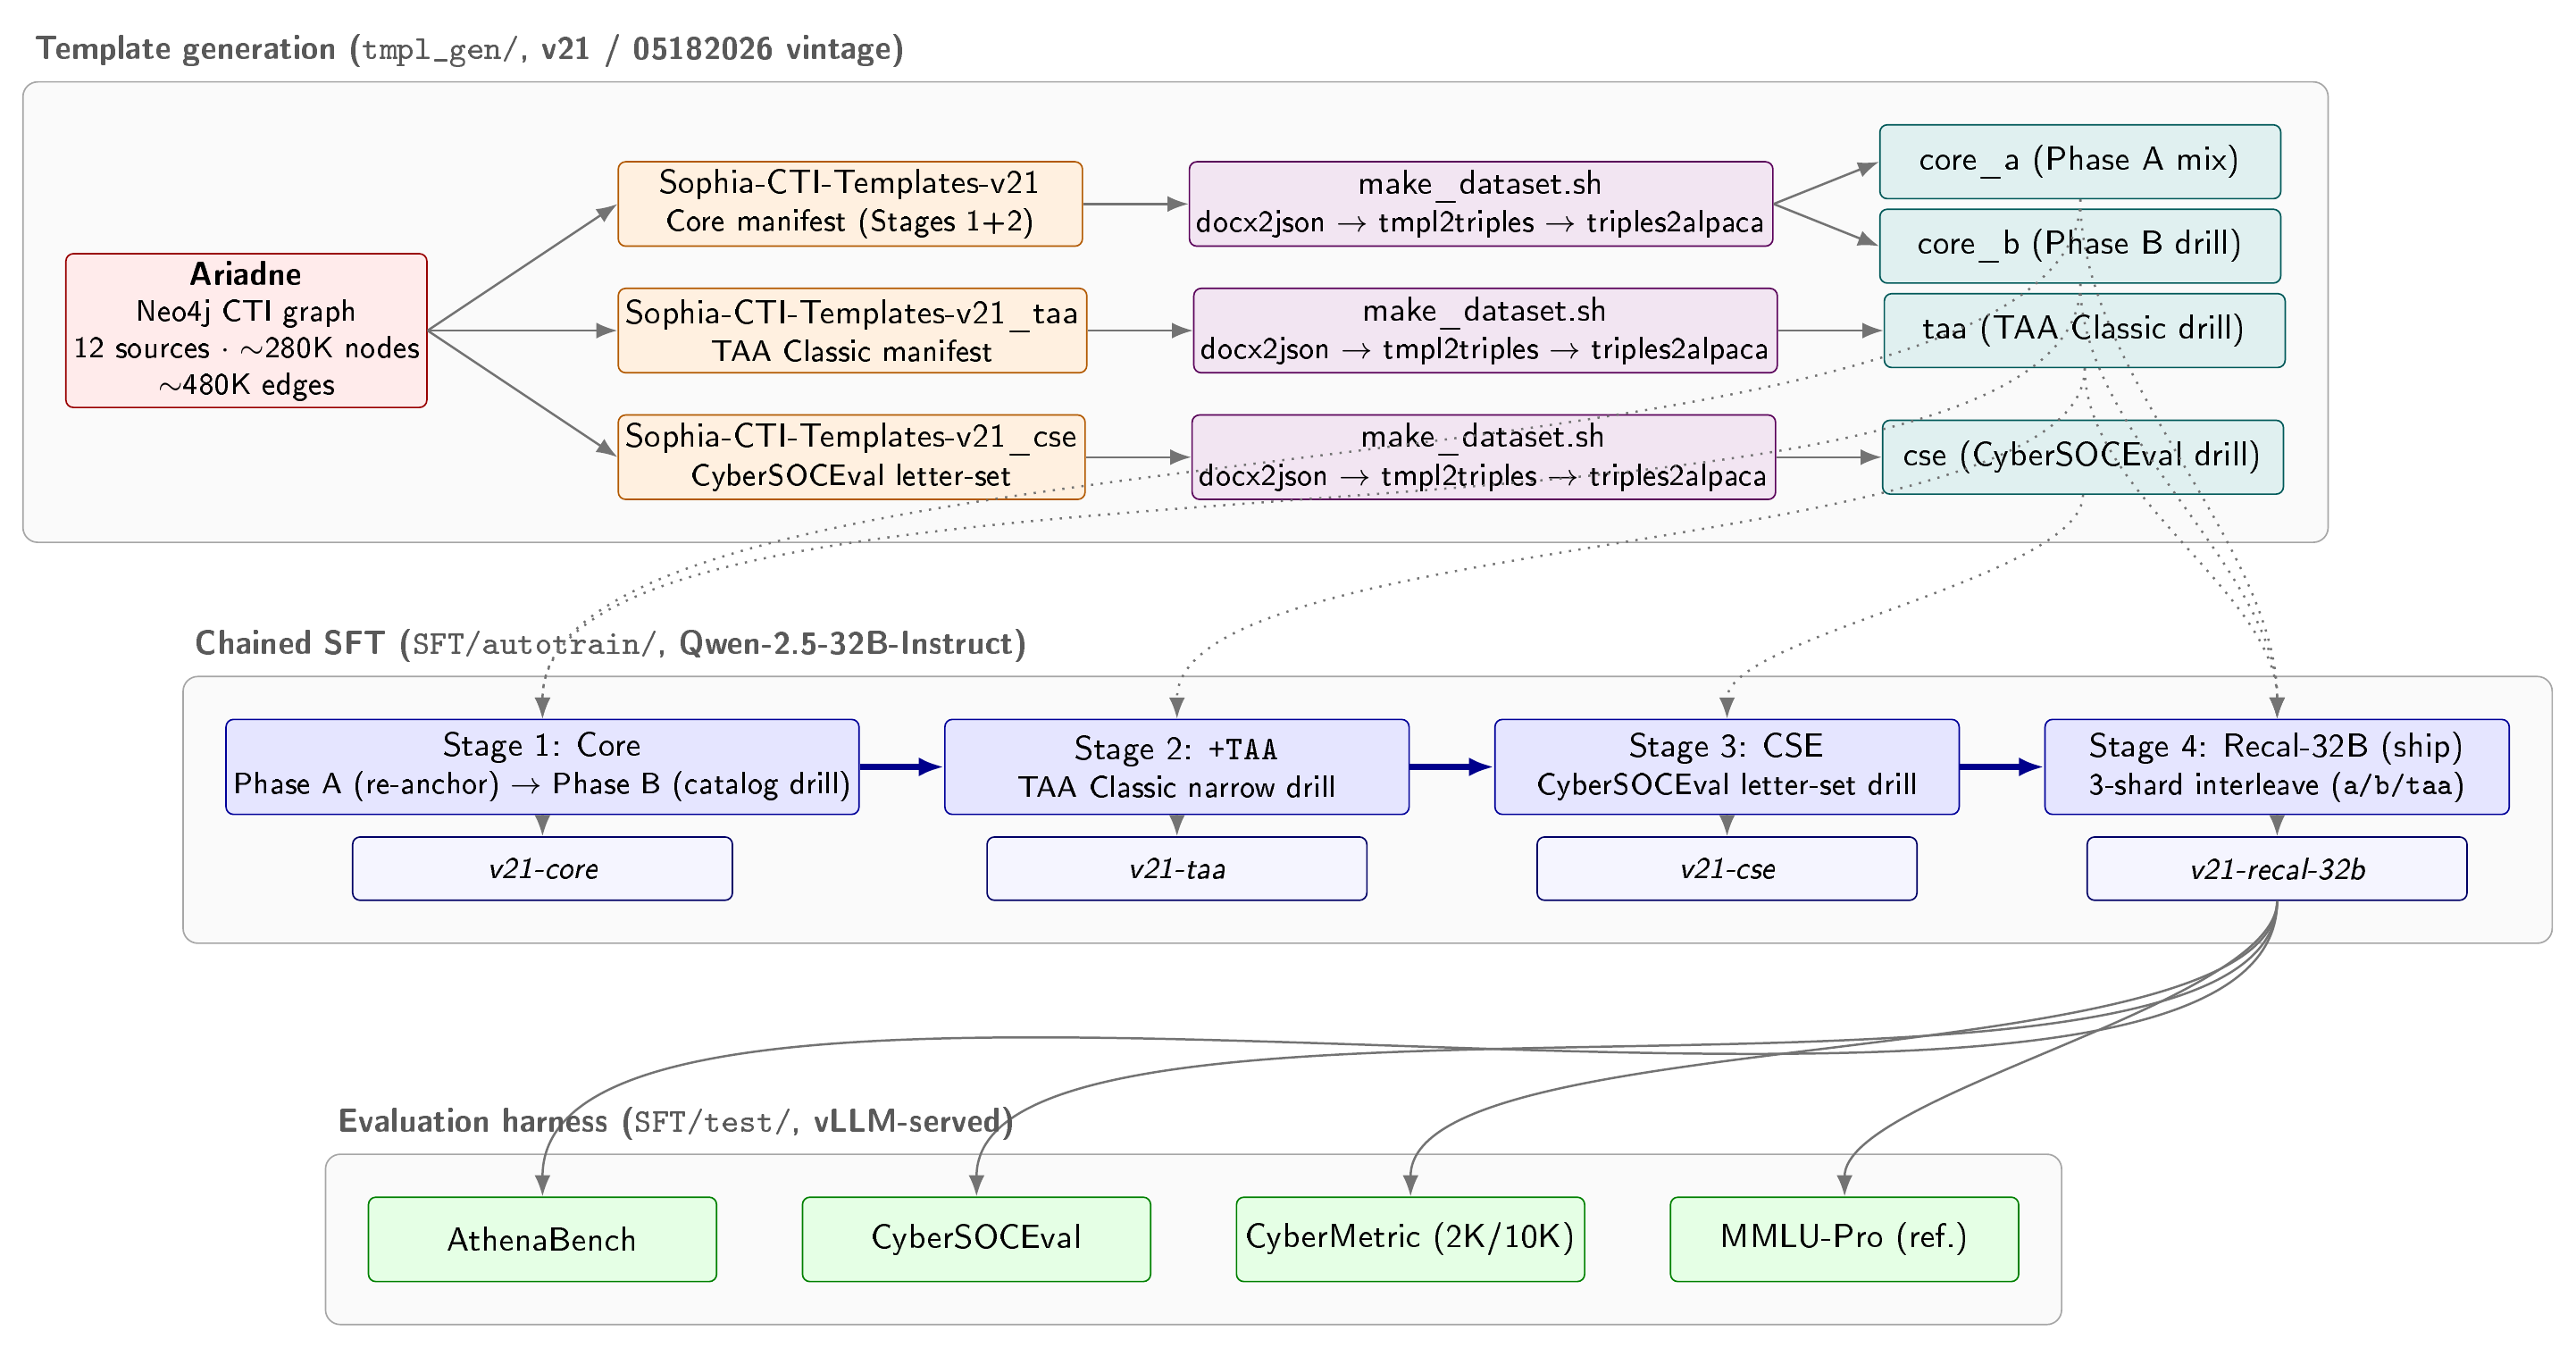
\includegraphics[width=\textwidth]{img/glaukopis_v21_flow.png}
\caption[]{\textbf{Glaukopis v21 end-to-end flow.} Ariadne (Section~\ref{sec:ariadne}), the Athena Neo4j CTI substrate, feeds three v21 template manifests---Core, TAA, and CSE---each processed by the \texttt{make\_dataset.sh} pipeline into Alpaca-format dataset shards. Four production shards (\texttt{core\_a}, \texttt{core\_b}, \texttt{taa}, \texttt{cse}; matched validation shards omitted for clarity) drive the four-stage chained SFT recipe targeting Qwen-2.5-32B-Instruct, producing the cumulative \texttt{v21-core}, \texttt{v21-taa}, \texttt{v21-cse}, and ship \texttt{v21-recal-32b} checkpoints. Dotted arrows mark which shards feed which stages; Stage~4 re-uses Core-A, Core-B, and TAA as a three-shard interleaved touch-up. Each pushed checkpoint is evaluated against the AthenaBench, CyberSOCEval, CyberMetric, and MMLU-Pro suites under a vLLM-served harness.}
\label{fig:glaukopis-v21-flow}
\end{figure*}

\paragraph{Reproducibility provenance.}
v21 is a strict reproducibility experiment on top of a predecessor vintage v18.1. The three Sophia-CTI template manifests, the row-count gate JSONs, and the per-stage count limits are \texttt{shasum}-verified byte-identical to their v18.1 sources; only dataset names, build-directory names, and Hugging Face push targets change between the two vintages. The v21 sign-off gate was that the post-Core checkpoint would land within $\pm 1.5$ percentage points of the v18.1 Core peak on every benchmark axis. The Total Score landed inside that band, but two per-axis sub-scores (ATE and RCM) drifted outside it, with the same shape that the intermediate v19 and v20 vintages had previously shown against v18.1. The most parsimonious explanation, given that the recipe-side inputs are byte-identical, is data-build non-determinism in the substrate sampler, dedup tiebreaks, and shuffle seeding inside \texttt{make\_dataset.sh}---a hypothesis confirmed by the fact that pinning the Neo4j read order and seeding the substrate sampler is the next-vintage research direction. The lineage discipline is in our judgement itself a contribution: by carrying byte-identical templates and gates forward across vintages, the Glaukopis pipeline isolates recipe drift from data-layer drift as separable failure modes, and provides a falsification matrix against which future vintages can be evaluated.

\paragraph{The off-plan Recalibrate stage.}
The v21 plan as originally specified was a three-stage chain (Core $\to$ +TAA $\to$ CSE). A recurring pattern observed across v18.1, v19, v20, and v21 chains is that Stage~3's narrow CyberSOCEval-letter-set drill reliably trades approximately ten percentage points of VSP for the CyberSOCEval-Malware lift it is designed to produce. To recover the VSP regression without sacrificing the Stage~3 gains, an off-plan fourth stage---\emph{Recalibrate}---was added as a three-shard interleaved touch-up over Core-A, Core-B, and TAA. At the 14B base scale, a single Recalibrate recipe (1e-6 LR, $0.25 / 0.40 / 0.35$ interleave probabilities, \texttt{--max-samples 2400}) cleanly recovers VSP. At the 32B base scale, the same recipe sits at the \texttt{adamw\_8bit} optimizer noise floor and drifts VSP the wrong way; the recipe was therefore re-tuned (3e-6 LR, $0.15 / 0.60 / 0.25$ Phase-B-heavy mix, \texttt{--max-samples 3600}) to expose more VSP/RMS catalog per interleaved row while holding step count and wall-time constant. The 32B Stage~4 split is the basis of the ship checkpoint discussed in Section~\ref{sec:glaukopis-sft}.

\paragraph{Architecture ports.}
Stages 1 through 3 carry the same recipe byte-identically across all five base-model ports of v21: Qwen-2.5-32B-Instruct (canonical), Qwen-2.5-14B-Instruct, Foundation-Sec-8B, Llama-3.1-8B-Instruct, and Qwen3-30B-A3B-Thinking-2507 (a thinking-mode MoE). The fact that the same template-baked shards drive all ports is what makes cross-architecture comparison meaningful: any axis-level differences between checkpoints derived from different bases under the same recipe and same data are attributable to base-model differences rather than training-data drift. The Qwen3-MoE port is also the first port to exercise a thinking-on / thinking-off A/B at serve time, exposing the SFT contribution to no-trace inference behavior separately from the base model's reasoning gain. Stage 4 is the only stage where the recipe does not carry identically across architectures: at the 32B dense scale the Phase-B-heavy 3e-6 LR variant is required (as discussed above), and on the Qwen3-MoE port Stage~4 closed without a beat against \texttt{v21-cse} on either Stage-4 variant, so the on-chain ship for that port is \texttt{v21-cse}.

\subsection{The Glaukopis SFT Chain}
\label{sec:glaukopis-sft}

The Glaukopis SFT pipeline is a four-stage chain over template-generated CTI instruction data. The canonical configuration targets Qwen-2.5-32B-Instruct as the base model and produces a sequence of four cumulative checkpoints---Core, +TAA, CSE, and Recalibrated-32B---of which the last is the production ship checkpoint. The same recipe ports byte-identically to four other base architectures (Qwen-2.5-14B-Instruct, Foundation-Sec-8B, Llama-3.1-8B-Instruct, and the Qwen3-30B-A3B-Thinking-2507 MoE), with only the base-model pointer and per-architecture memory flags changing between ports. The four-stage structure is itself the load-bearing element of the recipe; the per-stage details are described below.

\paragraph{Dataset shards.}
The chain consumes seven dataset shards produced by the template generator. The \textbf{Core-A} shard is a broad re-anchor mix combining knowledge-base, multiple-choice, threat-actor-attribution (TAA), SOC-style, CyberMetric-style, mitigation-strategy, and yes/no instruction families. The \textbf{Core-B} shard is an AthenaBench catalog drill targeting Risk Mitigation Strategy (RMS), Attack Technique Extraction (ATE), Vulnerability Severity Prediction (VSP), and Root Cause Mapping (RCM) tasks \cite{alam2025athenabench}. The \textbf{TAA} shard is a narrow drill on TAA Classic. The \textbf{CSE} shard is a CyberSOCEval letter-set drill, structured to exercise the format and reasoning pattern used by the CyberSOCEval malware and threat-intel test suites \cite{cybersoceval2025}. Three matched validation shards (\textbf{Core-Val}, \textbf{TAA-Val}, \textbf{CSE-Val}) hold out a per-axis slice (50 rows per shortname) for held-out evaluation during training. All shards are template-baked and therefore architecture-independent: a single set of seven JSON files feeds every base-model port.

\paragraph{Stage 1: Core (broad re-anchor + AthenaBench catalog drill).}
Stage 1 runs as two phases inside a single launcher, with only the final phase's merged checkpoint pushed. \emph{Phase A} is the broad re-anchor: it trains on the Core-A shard together with a general-purpose instruction mix (the Tülu-3 SFT mixture and an Alpaca-English demonstration set) at sequence length 8\,192, packing on, learning rate $1 \times 10^{-5}$, and effective batch size 16. The intent is to re-establish broad instruction-following behavior on top of a CTI vocabulary base. \emph{Phase B} drills on the Core-B AthenaBench-catalog shard at sequence length 16\,384 with packing off (so that long structured outputs are not truncated by packing boundaries), learning rate $5 \times 10^{-6}$, and effective batch size 8. The shorter, lower-LR Phase B is calibrated to imprint precise AthenaBench task structure on top of the broad foundation laid by Phase A, rather than to continue broad assimilation \cite{alam2025athenabench}. Together, Phase A and Phase B implement at fine granularity the principle from FLAN-T5 and ``Don't Stop Pretraining'' that broad domain exposure and narrow task supervision benefit from separate optimization regimes \cite{chung2022flant5,gururangan2020dontstop}.

\paragraph{Stage 2: +TAA narrow drill.}
Stage 2 takes the Core checkpoint as its base and trains on the TAA shard alone, at sequence length 4\,096, packing on, learning rate $5 \times 10^{-6}$, and effective batch size 16. The objective is to harden the model's TAA Classic performance without disturbing the broader catalog skills established in Stage 1.

\paragraph{Stage 3: CSE letter-set drill.}
Stage 3 takes the +TAA checkpoint and trains on the CSE shard at the same sequence length, packing, learning rate, and effective batch size as Stage 2. This stage is targeted preparation for the CyberSOCEval malware and threat-intelligence suites \cite{cybersoceval2025}, and is the point at which a known trade-off appears: lifting the CyberSOCEval axis through this drill comes at a measured cost to VSP performance from Stage 1's Phase B, which the next stage exists to recover.

\paragraph{Stage 4: Recalibrated touch-up (ship variant).}
Stage 4 is a three-shard interleaved touch-up trained off the Stage 3 (CSE) checkpoint with the explicit goal of recovering the VSP regression introduced by Stage 3 without losing Stage 3's CyberSOCEval gains. The ship variant trains on a Core-A / Core-B / TAA mix at relative sampling probabilities $0.15 / 0.60 / 0.25$ (i.e., Phase-B-heavy), using LlamaFactory's \texttt{interleave\_under} mixing strategy with a 3\,600-row sample cap, at sequence length 16\,384, packing off, learning rate $3 \times 10^{-6}$, and effective batch size 8. The 14B-tuned variant of this recipe (lower learning rate, more balanced mixture, smaller sample cap) is retained as a recipe-provenance A/B against the ship-grade 32B recipe, but in the 32B-target chain it is the higher-LR, Phase-B-heavy variant that recovers VSP and tops the v21 evaluation leaderboard.

\paragraph{Cross-cutting training-system details.}
All four stages share the same systems-level configuration: bf16 mixed precision, DeepSpeed ZeRO-3 (with optional CPU offload), the \texttt{adamw\_8bit} optimizer (mandatory at the 32B scale to fit activations), Liger kernels for fused attention paths, and gradient checkpointing on at 32B regardless of GPU count. The 8$\times$H100-80GB SXM topology is the canonical training target; 8$\times$H200-141GB SXM and 8$\times$RTX-PRO-6000-96GB are supported alternates. Effective batch size is held constant across launch topologies by auto-scaling gradient accumulation to GPU count.

\paragraph{Why four stages rather than one.}
The four-stage structure embodies the chained-SFT rationale from Section~\ref{sec:intro-chained-sft} in a CTI-specific form. Stages 1A and 1B separate broad domain absorption from precise structured-task imprinting, each at its own learning rate and packing regime \cite{gururangan2020dontstop,chung2022flant5}. Stages 2 and 3 carry out narrow drills against specific benchmark axes (TAA and CyberSOCEval respectively) without re-perturbing the broader skill set learned in Stage 1. Stage 4 is a recalibration step that recovers regressed axes (here, VSP) through controlled three-shard interleaving and a slightly higher learning rate, exploiting the fact that all template-generated shards remain available as training corpora throughout the chain. The result is a sequence of intermediate checkpoints---Core, +TAA, CSE, Recalibrated-32B---that can each be evaluated independently against the benchmark portfolio of Section~\ref{sec:benchmarks}, supporting controlled per-stage ablation in addition to producing a single ship checkpoint. This per-stage observability is itself a benefit of the chained structure: any axis-level regression observed at evaluation time is attributable to a specific stage and a specific dataset shard, and can be addressed by re-running only the affected stages rather than the full pipeline.

\subsection{Evaluation Harness}
\label{sec:glaukopis-eval}

Each pushed checkpoint in the Glaukopis chain is evaluated against the portfolio described in Section~\ref{sec:benchmarks}, consisting of \textbf{AthenaBench} (the six CTI tasks: CKT/MCQ, RCM, VSP, ATE, TAA Classic and Canonical, and RMS) \cite{alam2025athenabench}; \textbf{CyberSOCEval} (the malware and threat-intelligence test suites) \cite{cybersoceval2025}; \textbf{CyberMetric} at the 2\,000- and 10\,000-question tiers \cite{tihanyi2024cybermetric}; and \textbf{MMLU-Pro} as a decoupled general-intelligence reference. Serving is via vLLM in an OpenAI-compatible configuration; the same alias-keyed harness scores public baselines through hosted inference providers for direct comparison. Per-task token and wall-clock usage is captured so that benchmark sweeps are accompanied by a cost summary covering both API and local-GPU compute, which lets evaluation cost be reported alongside accuracy as a first-class metric.

The mapping between training stages and evaluation suites is deliberate: AthenaBench RMS/ATE/VSP/RCM are exercised by Stage 1 Phase B's Core-B shard; AthenaBench TAA Classic and TAA Canonical are exercised by Stage 2; CyberSOCEval malware and threat-intel reasoning are exercised by Stage 3; CyberMetric and the AthenaBench MCQ axis are exercised primarily by Stage 1 Phase A's Core-A shard. The Stage 4 recalibration is designed not to alter this mapping but to recover any axis that has regressed across the prior stages, with the 32B-tuned, Phase-B-heavy mixture specifically chosen to restore VSP without sacrificing CyberSOCEval performance. MMLU-Pro is run on a separate session so that suite scope stays decoupled from CTI scoring: it is reported as a sanity check on general capability rather than as a target for optimization.

\subsection{Toward Cyber Security Expert Small Language Models}
\label{sec:glaukopis-expert-slm}

Bringing together the elements above, an end-to-end cyber security expert SLM pipeline of the kind exemplified by Glaukopis can be summarized as:

\begin{enumerate}
  \item \textbf{CTI graph construction.} Continuously ingest and normalize CTI sources (ATT\&CK, CVE, CAPEC, CWE, ENGAGE, ICS/OT sources, proprietary feeds) into a Neo4j or similar graph.
  \item \textbf{Template authoring.} CTI experts encode important reasoning patterns (knowledge recall, root cause mapping, severity estimation, attribution clues, mitigation reasoning) as templates in the Athena language.
  \item \textbf{IFT generation.} Run the generation tool with version and date constraints aligned to a training window, producing large, structured IFT datasets per task family \cite{cardei2025ift}.
  \item \textbf{Chained SFT.} Fine-tune SLMs (e.g., 8--32B open models) using a chain of stages as described in Section~\ref{sec:glaukopis-sft}, with the dataset-shard / stage mapping aligned to the benchmark portfolio.
  \item \textbf{Evaluation.} Benchmark models on AthenaBench, CyberSOCEval, CyberMetric, and complementary suites (CTIBench, SecEval, CyberBench, SEvenLLM-Bench) to assess generalization and compare with larger proprietary models \cite{alam2024ctibench,alam2025athenabench,hu2024seceval,liu2024cyberbench,ji2024sevenllm,tihanyi2024cybermetric,cybersoceval2025}.
  \item \textbf{Feedback and iteration.} Use benchmark error patterns to design new templates, adjust CTI graph coverage, or refine IFT data (e.g., adding more negative cases or multi-hop chains), and re-run only the affected SFT stages.
\end{enumerate}

This pipeline is closely aligned with IBM's vision of cyber security expert SLMs \cite{levi2024cyberpal,levi2025toward}, but anchored in Athena's graph-driven IFT, the chained-SFT recipe described above, and dynamic CTI benchmarking via AthenaBench and CyberSOCEval.


\section{Results}
\label{sec:results}

This section reports the evaluation of the v21 Glaukopis vintage against the benchmark portfolio of Section~\ref{sec:benchmarks}: AthenaBench (six tasks: CKT, ATE, RCM, RMS, VSP, and TAA, with TAA scored as the combined-form average across Classic and Canonical), CyberSOCEval (Malware-analysis and Threat-Intel-Reasoning subsets), CyberMetric at the 2\,000- and 10\,000-question tiers, and MMLU-Pro as a decoupled general-intelligence reference. All numbers in this section come from the same harness run (sweep dated 2026-05-24), use the same vLLM serving stack for local checkpoints, and use the same hosted-API endpoints for public-model baselines.

\subsection{Three Averaging Schemes and Why MMLU-Pro Is Reported Separately}
\label{sec:results-averaging}

Because the three CTI benchmarks differ substantially in their internal structure---AthenaBench has six tasks, CyberSOCEval has two, and CyberMetric has two tiers---there is no single canonical way to aggregate them into a summary number, and the choice of aggregation visibly changes the leaderboard. We therefore report three averages for every model:

\begin{itemize}
  \item \textbf{Avg CTI Benchmark Score.} The unweighted mean of three per-benchmark summaries: AthenaBench (combined), CyberSOCEval (combined), and CyberMetric (2K+10K average). Each benchmark contributes equal weight regardless of how many internal tests it contains. This is the closest analogue to how published leaderboards typically present cyber LLM results and is the score we use for cross-benchmark comparison.
  \item \textbf{Avg CTI Test Score.} The unweighted mean across the ten individual CTI tests---six AthenaBench tasks, two CyberSOCEval subsets, and the two CyberMetric tiers---giving each test equal weight. This view is sensitive to the internal structure of each benchmark: AthenaBench, with six tests, exerts more pull on the score than CyberSOCEval or CyberMetric, which have two tests each. It is the most informative when the goal is to compare aggregate per-task capability.
  \item \textbf{Avg Total Test Score (with MMLU-Pro).} The same per-test average as above, but extended to include MMLU-Pro. MMLU-Pro is a general-intelligence reference and is \emph{not} part of the CTI use case we ultimately care about; we report this third average chiefly to quantify how much general capability each SFT run has traded away for CTI specialization---a ``forgetting'' diagnostic rather than a target for optimization.
\end{itemize}

The three averages tell complementary stories. The per-benchmark average is the most charitable view for SFT models, because it rewards strong performance on benchmarks whose internal structure aligns with the training data (here, AthenaBench). The per-test average reweights toward AthenaBench's six tasks but is invariant to how those tasks are pooled, making it the most apples-to-apples cross-architecture metric. The MMLU-Pro-augmented average is informative only as a counterpoint: SFT'd models systematically lose MMLU-Pro relative to their bases, and the magnitude of that loss is a useful diagnostic for the cost of specialization.

\paragraph{Note on cost figures.}
A per-evaluation cost analysis is in preparation alongside this manuscript. Costs are tracked end-to-end by the evaluation harness for both hosted-API models (token-priced via the published rate card of each provider) and local checkpoints (wall-clock $\times$~GPU rate on the 2$\times$H100 reference host). The cost numbers reported in Section~\ref{sec:results-cost} are draft and subject to refinement before final submission; the headline accuracy and capability findings are stable.

\subsection{Headline Comparison: v21 Ship Checkpoint vs.\ Frontier Reference Points}
\label{sec:results-headline}

Table~\ref{tab:results-headline} compares the Glaukopis v21 ship checkpoint, \texttt{athena-cti-sft-qwen25-32b-v21-recal-32b}, against its base instruct model and against six frontier-class reference points spanning the major proprietary and open-weights frontier families. All three averages are reported alongside the underlying per-benchmark scores. Three observations:

\begin{enumerate}
  \item \textbf{Chained SFT adds 7.3 points of average CTI benchmark capability over the base Qwen-2.5-32B-Instruct} (59.0 $\to$ 66.3) without changing the parameter count or runtime footprint. On the per-test average the lift is even larger (49.6 $\to$ 62.9, +13.3 points), because the per-test average gives full weight to AthenaBench's six tasks, on which the chain is explicitly trained. The largest single-axis lift is on AthenaBench combined (44.2 $\to$ 66.5; +22.3 absolute).
  \item \textbf{The ship checkpoint approaches frontier-class CTI performance.} On Avg CTI Benchmark Score the v21 ship sits within 4--7 points of the leading frontier models (GPT-5.5 at 72.9, DeepSeek-V4-Pro at 70.4, Gemini-3-Flash-Preview at 69.8), and is closely competitive with mid-tier frontier offerings (GPT-5.2 at 67.5, DeepSeek-v3.2-Exp at 66.0). On Avg CTI Test Score the same pattern holds (62.9 vs.\ leaders at 67--73). It is competitive with Gemini-2.5-Flash on both averages despite the substantial parameter-count gap.
  \item \textbf{Catastrophic forgetting in the MMLU-Pro dimension is real, but not unique to Glaukopis and not a target for optimization.} MMLU-Pro drops from 69.0 (Qwen-2.5-32B-Instruct base) to 57.4 (v21 ship), an 11.6-point absolute regression that reflects the well-known cost of domain specialization. The Avg Total Test Score (with MMLU-Pro) figure makes this explicit: the v21 ship at 62.8 trails GPT-5.5 (76.9) by a wider margin on this composite than on either CTI-only average. Because MMLU-Pro is not part of the CTI use case we ultimately care about, this regression is reported as a diagnostic rather than treated as a metric to optimize against; we discuss possible mitigations in Section~\ref{sec:open-challenges}.
\end{enumerate}

\begin{table*}[t]
\centering
\caption{Headline results: Glaukopis v21 ship checkpoint vs.\ base model and frontier reference points. Three averages are reported per the schemes defined in Section~\ref{sec:results-averaging}: \textbf{Avg CTI Bench} (3 benchmarks, equal weight), \textbf{Avg CTI Test} (10 CTI tests, equal weight), and \textbf{Avg Total (w/MMLU)} (10 CTI tests plus MMLU-Pro). All numbers from the 2026-05-24 evaluation sweep. AB Avg II is the AthenaBench composite using the 50/50 TAA Classic+Canonical blend.}
\label{tab:results-headline}
\small
\setlength{\tabcolsep}{4pt}
\begin{tabular}{lcccccccc}
\hline
\textbf{Model} & \textbf{Type} & \textbf{Avg CTI} & \textbf{Avg CTI} & \textbf{Avg Total} & \textbf{AB Avg} & \textbf{CSE} & \textbf{CM} & \textbf{MMLU-} \\
               &               & \textbf{Bench}   & \textbf{Test}    & \textbf{(w/MMLU)}  & \textbf{II}    & \textbf{comb} & \textbf{avg} & \textbf{Pro} \\
\hline
GPT-5.5                                  & Frontier  & 72.9 & 73.5 & 76.9 & 77.0 & 48.3 & 93.3 & 88.3 \\
DeepSeek-V4-Pro                          & OS-PT     & 70.4 & 67.9 & 69.6 & 67.2 & 52.2 & 91.8 & 79.1 \\
Gemini-3-Flash-Preview                   & Frontier  & 69.8 & 68.4 & 71.7 & 69.3 & 48.1 & 92.1 & 89.2 \\
GPT-5.2 (reasoning=medium)               & Frontier  & 67.5 & 65.0 & 67.0 & 63.8 & 46.8 & 91.8 & 81.3 \\
DeepSeek-v3.2-Exp                        & OS-PT     & 66.0 & 62.2 & 63.9 & 59.0 & 47.2 & 91.7 & 82.5 \\
\textbf{v21-recal-32b (ship)}            & SFT       & \textbf{66.3} & \textbf{62.9} & \textbf{62.8} & \textbf{66.5} & 42.6 & 89.8 & 57.4 \\
v21-cse                                  & SFT       & 65.8 & 62.4 & 62.2 & 66.6 & 42.0 & 88.8 & 54.2 \\
v21-recalibrate (14B-recipe)             & SFT       & 65.9 & 62.4 & 62.2 & 65.9 & 42.4 & 89.2 & 54.6 \\
Gemini-2.5-Flash                         & Frontier  & 63.4 & 57.9 & 59.8 & 53.1 & 46.2 & 91.0 & 82.1 \\
v21-core                                 & SFT       & 62.6 & 61.6 & 63.2 & 67.2 & 31.1 & 89.6 & 59.2 \\
v21-taa                                  & SFT       & 62.0 & 61.7 & 63.7 & 66.9 & 29.8 & 89.4 & 58.2 \\
Qwen2.5-32B-Instruct (base)              & Instruct  & 59.0 & 49.6 & 49.3 & 44.2 & 42.6 & 90.2 & 69.0 \\
\hline
\end{tabular}
\end{table*}

\paragraph{Why \texttt{v21-recal-32b} is the ship checkpoint, not \texttt{v21-recalibrate}.}
The two Stage-4 variants warrant brief comparison because they share the same Stage-3 parent (\texttt{v21-cse}) and differ only in the Stage-4 recipe. \texttt{v21-recalibrate} runs the 14B-tuned Stage-4 recipe verbatim on the 32B base (learning rate $1\times 10^{-6}$, balanced 0.25/0.40/0.35 interleave probabilities, \texttt{--max-samples 2400}); \texttt{v21-recal-32b} runs the recipe re-tuned for the 32B parameter scale (learning rate $3\times 10^{-6}$, Phase-B-heavy 0.15/0.60/0.25 mix, \texttt{--max-samples 3600}). On the headline aggregates the two variants are within 0.5 points of each other (Avg CTI Bench 66.3 vs.\ 65.9; Avg CTI Test 62.9 vs.\ 62.4), which on its own would not be enough to prefer one over the other. The deciding factor is per-axis: \texttt{v21-recal-32b} restores VSP to 77.8 against \texttt{v21-recalibrate}'s 75.7, and that VSP recovery is precisely what Stage~4 is for at the 32B scale (Section~\ref{sec:glaukopis-v21-templates}). The 14B-recipe variant sits at the \texttt{adamw\_8bit} optimizer noise floor at 32B---enough to nudge most axes in the right direction, but not enough to recover the VSP regression introduced by Stage~3. \texttt{v21-recal-32b} is therefore the recommended ship checkpoint at the 32B scale, with \texttt{v21-recalibrate} retained on disk as the recipe-provenance A/B against it.

\subsection{Per-Stage Ablation: What Each SFT Stage Contributes}
\label{sec:results-per-stage}

Because the Glaukopis chain pushes a Hugging Face checkpoint after every stage, the per-stage contribution to each benchmark axis is directly measurable. Table~\ref{tab:results-per-stage} reports the AthenaBench axis breakdown for the Qwen-2.5-32B chain alongside the base model, decomposing how Core $\to$ +TAA $\to$ CSE $\to$ Recalibrate-32B accumulates capability.

The data confirm the design rationale of the chain (Section~\ref{sec:glaukopis-sft}):

\begin{itemize}
  \item \textbf{Stage 1 (Core) does most of the AthenaBench-catalog work.} The Phase~B catalog drill lifts ATE from 18.2 (base) to 67.2 (Core), RMS combined-f1 from 7.6 to 63.8, and RCM from 59.5 to 69.8. These are the gains the rest of the chain must preserve.
  \item \textbf{Stage 2 (+TAA) introduces meaningful Canonical-TAA capability.} TAA Canonical combined rises from 2.0 (base) and 18.4 (Core) to 36.8 at +TAA, the largest single-stage Canonical lift in the chain.
  \item \textbf{Stage 3 (CSE) lifts the CyberSOCEval axis} from 31.1 (Core) to 42.0 (CSE), a +10.9 absolute gain. The expected VSP trade-off is also visible: VSP drops from 83.1 (Core) to 78.9 (CSE), consistent with the regression pattern observed across v18.1, v19, v20, and v21 (Section~\ref{sec:glaukopis-v21-templates}).
  \item \textbf{Stage 4 (Recalibrate-32B) is recovery, not novel capability.} On the headline Avg CTI score the ship checkpoint at 66.3 is essentially tied with the post-CSE checkpoint at 65.8 and the 14B-recipe recalibrate variant at 65.9; the Stage~4 lift comes from re-aligning VSP (77.8) and stabilizing the CyberSOCEval combined score (42.6) rather than from new capability development.
\end{itemize}

\begin{table*}[t]
\centering
\caption{Per-stage AthenaBench breakdown for the Qwen-2.5-32B v21 chain (combined-form scores where multiple forms are released). Stage 1 (Core) does most of the AthenaBench-catalog work; Stage 2 introduces Canonical TAA; Stage 3 lifts CyberSOCEval; Stage 4 recovers VSP without losing prior gains.}
\label{tab:results-per-stage}
\small
\begin{tabular}{lcccccccc}
\hline
\textbf{Checkpoint} & \textbf{CKT} & \textbf{ATE} & \textbf{RCM} & \textbf{RMS} & \textbf{VSP} & \textbf{TAA Cl.} & \textbf{TAA Can.} & \textbf{AB II} \\
\hline
Qwen2.5-32B-Instruct (base) & 52.9 & 18.2 & 59.5 & 7.6  & 78.8 & 48.0 & 2.0  & 44.2 \\
v21-core                    & 72.9 & 67.2 & 69.8 & 63.8 & 83.1 & 46.5 & 18.4 & 67.2 \\
v21-taa                     & 75.4 & 63.4 & 69.0 & 62.9 & 83.5 & 47.0 & 36.8 & 66.9 \\
v21-cse                     & 72.5 & 63.4 & 67.7 & 63.7 & 78.9 & 53.5 & 3.4  & 66.6 \\
\textbf{v21-recal-32b}      & 75.5 & 65.8 & 67.1 & 62.5 & 77.8 & 50.5 & 3.4  & \textbf{66.5} \\
\hline
\end{tabular}
\end{table*}

\subsection{Cross-Architecture Ports: Recipe Transfer}
\label{sec:results-arch-ports}

The same v21 recipe ports byte-identically to four other base architectures, with only the base-model pointer and per-architecture memory flags changing between ports (Section~\ref{sec:glaukopis-v21-templates}). Table~\ref{tab:results-architectures} compares the best v21 SFT checkpoint produced by each port against its corresponding instruct base, reporting all three averages plus MMLU-Pro alongside the per-test lift.

\begin{table*}[t]
\centering
\caption{Cross-architecture v21 ports. \emph{Best v21}: highest-scoring SFT checkpoint for that base architecture on Avg CTI Benchmark Score. \textbf{Avg CTI Bench} and \textbf{Avg CTI Test} are the per-benchmark and per-test schemes defined in Section~\ref{sec:results-averaging}. \emph{$\Delta$ test} and \emph{$\Delta$ MMLU}: absolute differences between the best SFT checkpoint and the corresponding instruct base on Avg CTI Test and MMLU-Pro respectively. The Qwen-2.5-32B dense port is the cross-architecture optimum on CTI; the Qwen3-MoE port leads on MMLU-Pro among SFT'd checkpoints but is more expensive to serve and benchmark.}
\label{tab:results-architectures}
\small
\setlength{\tabcolsep}{4pt}
\begin{tabular}{llccccc}
\hline
\textbf{Base architecture}  & \textbf{Best v21 checkpoint} & \textbf{Avg CTI} & \textbf{Avg CTI} & \textbf{$\Delta$ test} & \textbf{MMLU-} & \textbf{$\Delta$ MMLU} \\
                            &                              & \textbf{Bench}   & \textbf{Test}    & \textbf{vs.\ base}     & \textbf{Pro}   & \textbf{vs.\ base}     \\
\hline
Qwen2.5-32B-Instruct        & v21-recal-32b   & \textbf{66.3} & \textbf{62.9} & +13.3 & 57.4 & $-$11.6 \\
Qwen2.5-14B-Instruct        & v21-recalibrate & 62.3 & 59.6 & +13.5 & 50.2 & $-$13.9 \\
Qwen3-30B-A3B-Thinking-2507 & v21-cse         & 63.4 & 60.9 &  +6.0 & 53.0 & $-$24.6 \\
Foundation-Sec-8B-Instruct  & v21-recalibrate & 53.8 & 53.2 &  +0.4 & 25.6 & $-$17.6 \\
Llama-3.1-8B-Instruct       & v21-recalibrate & 50.5 & 50.8 &  +7.3 & 27.7 & $-$20.6 \\
\hline
\end{tabular}
\end{table*}

Three cross-architecture observations are worth noting:

\begin{itemize}
  \item \textbf{Recipe transfer scales with base-model size, with one notable exception.} The 14B and 32B dense Qwen ports both show clear SFT lift over their bases (+13.5 and +13.3 on Avg CTI Test respectively), and the Llama-3.1-8B port also lifts well (+7.3). The Qwen3-MoE port shows a smaller lift (+6.0), and the Foundation-Sec-8B port barely moves (+0.4)---its base is already a security-specialized instruct release, so most of the gain Glaukopis would otherwise deliver is already present in the starting point. At the 8B scale generally, the v21 recipe is not the right shape; the next-vintage research direction includes recipe variants tuned specifically for that parameter range.
  \item \textbf{The Qwen3-MoE port leads on MMLU-Pro among SFT'd checkpoints, but is not the recommended ship.} \texttt{athena-cti-sft-qwen3-30b-a3b-thinking-2507-v21-cse} reaches Avg CTI Bench of 63.4 (within 3 points of the dense-32B ship) and retains MMLU-Pro at 53.0---4.4 points below the dense-32B ship's MMLU-Pro of 57.4 but the highest MMLU-Pro among any SFT'd Glaukopis checkpoint that is not the bare 32B. However, MMLU-Pro is a general-intelligence reference and is not part of the CTI use case we ultimately care about (Section~\ref{sec:results-averaging}). On the CTI averages that do matter, the dense Qwen-2.5-32B port wins; it is also substantially less expensive to serve and benchmark than the MoE port (the MoE's 128-expert top-8 routing is more expensive both per token and end-to-end through the evaluation harness). The dense Qwen-2.5-32B port is therefore the most efficient and most CTI-capable production ship for the use cases at hand.
  \item \textbf{MMLU-Pro regression varies by port and is largest at the smaller scales.} The dense 32B port loses 11.6 points of MMLU-Pro, the 14B port loses 13.9, the MoE port loses 24.6, and the 8B ports lose 17.6--20.6. At the 32B Qwen scale the regression is the most contained in absolute terms, which is part of why that port is the recommended ship.
\end{itemize}

\subsection{Cost Analysis (Draft)}
\label{sec:results-cost}

\paragraph{Status.}
A per-evaluation cost analysis is being finalized alongside this manuscript. The cost-tracking instrumentation captures, for every model and every benchmark suite, (i) input and output token counts and the relevant per-1K-token rate card for hosted-API checkpoints, and (ii) wall-clock seconds and a per-GPU-hour rate ($\$2.50$/GPU-hour on the 2$\times$H100 reference host) for locally-served vLLM checkpoints. These are blended into a single cost-per-full-suite-evaluation figure that lets accuracy be reported alongside cost as a first-class metric.

\paragraph{Preliminary observations.}
The draft cost figures support the broad shape of the argument advanced in the Introduction: on a full-suite evaluation pass (AthenaBench + CyberSOCEval + CyberMetric 2K+10K + MMLU-Pro), the leading frontier proprietary models cost between approximately \$160 and \$1{,}150, the strongest open-weights frontier models cost between approximately \$11 and \$130, and the locally-served Glaukopis v21 32B ship checkpoint costs approximately \$3 at the reference 2$\times$H100 hourly rate. The cost ratio between the v21 ship and the leading proprietary frontier is therefore between two and three orders of magnitude per evaluation pass at the time of writing, with the v21 ship landing within a few points of the frontier on Avg CTI Benchmark Score. A finalized cost table with model-by-model break-downs and standardized denominators (per-prompt, per-token, per-evaluation-pass) will appear in this section in the camera-ready version.

\paragraph{Why the cost ratio matters.}
Two reasons, both already developed in the Introduction. First, regulated SOC environments have hard limits on what can be sent to a third-party API; locally-served Glaukopis 32B is a deployment-feasible artifact in those environments while the frontier models are not. Second, even where the legal posture allows API use, the per-evaluation cost ratio compounds across analyst workloads---a SOC running thousands of CTI lookups per day cannot afford the frontier pricing the leaderboard reflects. A 32B local checkpoint that closes most of the gap therefore changes the practical deployment calculus, even when the absolute capability gap to the frontier is real.


\section{Open Challenges and Research Directions}
\label{sec:open-challenges}

Despite rapid progress, several open questions remain:

\begin{itemize}
  \item \textbf{Data leakage and benchmark freshness.} Dynamic benchmarks like AthenaBench reduce, but do not eliminate, the risk that training data (e.g., from the same CTI sources) overlaps heavily with evaluation samples. Careful time-based splits and provenance tracking between the IFT generator and benchmarks will be crucial \cite{alam2025athenabench,cardei2025ift}.
  \item \textbf{Balancing symbolic templates and LLM creativity.} Template-based generation offers precision and coverage, but LLM-generated paraphrases can increase linguistic diversity and realism (e.g., multiple phrasings of the same CTI scenario). Hybrid pipelines that use templates to define semantics and LLMs to diversify surface form---while preserving correctness---are a promising area.
  \item \textbf{Incorporating chain-of-thought and explanations.} SecKnowledge~2.0 shows that CoT rationales significantly improve cyber reasoning \cite{levi2025toward}. Extending Athena templates to generate structured reasoning steps (via explicit graph traversal reasoning) and then augmenting them with LLM-generated natural language CoT could yield explainable CTI SLMs.
  \item \textbf{Operational evaluation dimensions.} AthenaBench focuses on knowledge and reasoning quality. Security operations also care about robustness to prompt injection, misuse, adversarial CTI, latency, and integration with SIEM/SOAR systems. Benchmarks like SecEval and CyberBench partly address this; extending AthenaBench and complementary suites to cover these aspects remains an important direction \cite{hu2024seceval,liu2024cyberbench,alam2025athenabench}.
  \item \textbf{Multilingual and cross-regional CTI.} SEvenLLM emphasizes bilingual corpora \cite{ji2024sevenllm}. Current CTI benchmarks primarily use English sources, omitting intelligence from other languages that often contain region-specific threats. Template-based IFT over multilingual CTI graphs and multilingual benchmark tasks could help close this gap.
  \item \textbf{Human-in-the-loop and analyst trust.} For high-stakes CTI decisions, analysts need to understand why the model suggested a mapping or mitigation and how it connects to CTI sources. Template-driven data, CTI graph citations, and CoT rationales may enable verifiable, inspectable explanations.
\end{itemize}

\section{Conclusion}

This paper has introduced Glaukopis, a methodology and a working system for producing small ($\le 32$B) cyber threat intelligence expert language models, and reported the v21 vintage's empirical evaluation against the AthenaBench, CyberSOCEval, CyberMetric, and MMLU-Pro suites. Three findings are central:

\begin{itemize}
  \item \textbf{Chained, template-grounded SFT delivers substantial CTI lift over a strong open base.} The v21 ship checkpoint adds 7.3 points on Avg CTI Benchmark Score and 13.3 points on Avg CTI Test Score over Qwen-2.5-32B-Instruct (59.0~$\to$~66.3 and 49.6~$\to$~62.9 respectively) without changing parameter count or runtime footprint, and the largest single-axis lift (AthenaBench combined, +22.3 absolute) lands precisely on the benchmark family the chain is designed around.
  \item \textbf{A 32B SFT'd model can approach frontier-class CTI performance at substantially lower per-evaluation cost.} The v21 ship sits within 4--7 average-CTI-benchmark points of the leading proprietary and open-weights frontier models---DeepSeek-V4-Pro, Gemini-3-Flash-Preview, GPT-5.5---at a small fraction of the per-evaluation cost. For regulated SOC environments where third-party API use is restricted, this changes the deployment calculus from ``frontier or nothing'' to ``frontier when allowed, on-premises 32B otherwise.''
  \item \textbf{The chained recipe is auditable and incrementally refreshable.} Because each stage pushes an intermediate checkpoint and consumes a specific dataset shard, per-axis regressions (e.g., VSP at Stage~3, MMLU-Pro across all stages) are attributable to specific stages and addressable by re-running only the affected ones. The v21 vintage's strict-reproducibility experiment over v18.1 additionally isolated data-build non-determinism in the template-generation substrate from recipe-level drift, informing the seed-pinning research direction for the next vintage.
\end{itemize}

The result is a principled and reproducible pathway from authoritative public CTI sources (via Ariadne), through a symbolic template language that turns those sources into instruction-tuning data, to a chained SFT recipe that produces deployable cyber security expert small language models grounded in CTI knowledge bases, instruction fine-tuning theory, and a rigorous benchmark portfolio. Glaukopis is one instantiation of that pathway; the broader argument it supports is that, for CTI workflows, on-premises 32B-scale models with disciplined SFT pipelines are a viable alternative to frontier proprietary models in deployment scenarios where the latter cannot in fact be deployed.


\section{Conflicts of interest}
None declared.

\section{Funding}
No external funding supported this manuscript.

\section{Data availability}
The Ariadne CTI knowledge graph is built from twelve public CTI sources listed in Section~\ref{sec:ariadne}; each is independently accessible from its original publisher and is downloaded and parsed by the open populator script described therein. The v21 template manifests, the seven IFT dataset shards, the per-stage SFT launchers, and the evaluation-harness wrappers used to produce the results in Section~\ref{sec:results} are maintained internally at Athena Security Group; release plans are under discussion. Cumulative HF checkpoints (\texttt{asg-ai/athena-cti-sft-qwen25-32b-v21-\{core,taa,cse,recal-32b\}} and the cross-architecture ports) are available on the Hugging Face Hub.

\section{Acknowledgments}
The authors thank colleagues at Florida Atlantic University's Department of Electrical Engineering and Computer Science and at Athena Security Group for discussions that informed this work.


\bibliographystyle{abbrvnat}
\bibliography{glaukopis-v1.1}

\end{document}
